\documentclass {article}
\usepackage{amsmath}
\usepackage{theoremref}
\usepackage{graphicx}
\graphicspath{ {images/} }

\title{Calculating a correct compiler using the Bahr and Hutton method}
\author{Marco Jones}

\begin{document}
\begin{titlepage}
    \begin{center}
        \vspace*{1cm}
        
        \Huge
         Calculating a correct compiler using the Bahr and Hutton method
        
        
        \vspace{2cm}
        \Large
        Marco Jones
        
       
        \vspace{1cm}
        \normalsize
        Supervisor: Colin Runciman
        
        \vspace{2.5cm}
        
                
        Project submitted in part fulfilment 
       for the degree of  BSc of  Computer Science \\

        \vspace{0.2cm}
   	University Of York\\
	\vspace{0.2cm}
 	26 April 2016
	
	\vspace{5cm}
	
	Word Count: 7991, as counted by TeXcount web interface:
	http://app.uio.no/ifi/texcount/online.php. 
	This includes the body of the report without the title page.
        
    \end{center}
\end{titlepage}

\tableofcontents
\clearpage

\newcommand{\BH}{Bahr and Hutton}
\newcommand{\vm}{virtual machine}

\section{Introduction}

Ever since the invention of electronic computers
the instruction set to operate them has grown massively.
At the lowest level, computers directly execute
a series of discrete binary electrical
pulses using logical circuits to perform computation.
These binary signals are far from random; they're formally
defined in a grammar, making it a \emph{language},
more specifically the language of ``Machine code'' instructions.
Managing operations in machine code is difficult on
a large scale,
so by abstracting away from the details of how a computer works,
 programmers have developed 
higher level programming languages;
these languages are easier for programmers to interpret
than machine code and that makes them much easier to use and bug fix.
However a computer still only understands machine code\footnote{
Assembly code can be executed by a computer 
with the use of an assembler,
which translates the assembly 
into machine code nonetheless.},
so clearly there is a gap to bridge in translating the 
\emph{source code} of a program, which can't be
executed, to machine code which can be executed.

There are two common approaches to making this translation:
interpretation and compilation, which are \emph{not mutually exclusive}, some languages use a mix of both 
strategies e.g. Python and C.

Interpretation involves using a
interpreter program which takes the abstract syntax of a
source program and immediately executes that to produce an output,
these languages are known as ``Interpreted'' languages.

In contrast there are compiled languages, these use 
a program called a compiler to translate the high level
source code into code of a lower level target language,
this target language is not necessarily machine code.
The end goal is to translate the source code into machine code
but there may be several intermediate languages in the process\cite[pg 8-10]{compilers}. Compiled languages tend to be more efficient
because the compiled code is easier the computer to translate
and execute rather than use another program to interpret
the source code on the conputers' behalf.

Compilers, like any program, need to go through testing to
verify functionality and expose bugs. However it
can be much more difficult to do this for compilers
because the bugs might not be in the implementation of 
compiler itself but the code that it may be able output.
Time can be saved in both testing and development
by merging the two; constructing a compiler
using mathematical rules and you can be more
assured of its correctness, this field is called
compiler calculation\cite{meijer}, 
but it's quite an
advanced topic; requiring a decent understanding 
of the formal mathematics behind it.

\BH\ have built upon these techniques and shown that
compiler calculation can be much simpler,
at least for compilers that produce code
for stack-based virtual machines.
The virtual machine takes the place of the
computer by executing code with a stack
to manipulate arguments, in a real computer
this can be likened to memory, in that
values are stored and manipulated in this space.

For a given source language, 
the \BH\ method produces
a compiler and corresponding \vm\
via equational reasoning,
with all of the definitions 
to compile source expressions
and the code to execute them,
emerging out of the calculation process.
Furthermore the method makes
use of structural recursion (where it can),
where the semantics of source expressions are defined
compositionally by the semantics of their arguments.
This allows the use of inductive methods
to derive definitions for the compiler and \vm\ efficiently
whilst simultaneously guaranteeing their correctness by virtue 
of \emph{constructive induction} \cite{backhouse},
without needing to specify how the 
machine should operate before hand.
The end result, is an equational program consisting of
definitions of the compiler and \vm,
and any axillary functions we create in the process.

\subsection{Aims and methodology}

The aim of this dissertation is to
see whether the \BH\ method can
be used to calculate a new and correct compiler
with a corresponding \vm, 
not defined in \BH's\ paper \cite{bandh}.
The compiler and \vm\ we will calculate 
will be for a source language which extends 
upon the Arithmetic language example\cite[Section 2]{bandh},
and will do so in three stages.

Firstly by summarising the \BH\ method,
using the arithmetic language derivation 
as described in, as a guide.

Secondly, the language will be gradually extended
by calculating new definitions of a more complex nature,
and implementing them in Haskell
\footnote{Haskell provides curried function application
		and explicit type declaration which are
		convenient for defining grammars,
		as consequence, the implementation closely
		resembles our calculations}.
Each extension of the language will be labelled 
as it's own language, it's compiler and \vm\ 
may appear in full in the summary of each section.
We will see the \BH\ method used to calculate
languages that include: eager and lazy conditionals, 
and variable bindings,
and although this project didn't get far enough
there will be discussion on the 
language of function declarations.

Each calculation we will be briefly tested
using an example expression
in three different ways.

\begin{enumerate}
	\item Compare hand compiled code against the
		implemented compiler.
	\item Compare results of hand executed code 
		against that of the \vm.
	\item Compare outputs of the \vm\ against the interpreter.
\end{enumerate}

Thirdly, we will use automated testing
to verify the definitions in the final
and most extended language; 
by construction, the automated
tests should verify all calculations up
to and including the 
should all tests pass, we will
be even more confident in our 
compiler's correctness.
The automated testing will all be in one section of it's own
near the end of this dissertation
because it will aim to test the end product compiler and \vm.
Moreover the language defined by this compiler and \vm\
can be thought of as a set union of every sub-languages,
therefore by transitivity, testing 
the whole set of languages together
also tests the individual functionality of every sub language.

Finally, we will conclude with 
reflection on using the \BH\ method,
and further work.

\subsection{Roadmap}

\S\ref{bhrev} will review the \BH\ method.
Because the whole project is based around a single
paper that describes it, there will be no review
of other literature.

In \S\ref{langcond} will see the extension of the compiler and
virtual machine with definitions for a conditional function

In \S\ref{langbind} the compiler and
virtual machine will be extended
 once more with definitions for variable declaration.
 
In \S\ref{langfunc} will be a discussion on what
would be expected of a compiler and \vm\ that
could handle function definition and application.

In \S\ref{autotesting} we will discuss the methods
of systematically testing the compiler and virtual machine.

\S\ref{conclusion} is the conclusion where there will
be reflection on the use of the \BH\ method and suggestions
for further work.

\pagebreak
\section{A review of the Bahr and Hutton method} \label{bhrev}

\BH\ begin their paper \S2.1 - \S2.4 of \BH's paper describe the unrefined 
method in detail, only to refine the process
in \S2.5 \cite[Combining the transformation steps]{bandh},
resulting in a much simpler 3 step process, 
this paper will only be concerned with
their refined 3 step method\cite[page 12]{bandh}.

\begin{enumerate}
	\item Define an evaluation function
		in a compositional manner.
	\item Define equations that specify
		the correctness of the compiler.
	\item Calculate definitions that 
		satisfy these specifications.
\end{enumerate}
\newcommand{\expr}{\textit{Expr}}

In \S2 they are deriving a compiler
and virtual machine for the ``Arithmetic'' language,
they begin by defining: a new Haskell data type \expr;
which contains the set of expressions which belong to their source language,
an evaluation function, also referred to as the \emph{interpreter},
which defines their semantics,
and a stack of integers where 
arguments are manipulated.
\newcommand{\eval}{\textit{eval}}
\newcommand{\val}{\textit{Val}}
\newcommand{\add}{\textit{Add}}
\newcommand{\code}{\textit{Code}}
\newcommand{\Val}{\mathit{Val\ }}
\newcommand{\Add}{\mathit{Add\ }}
\newcommand{\evalf}{\mathit{eval\ }}
\newcommand{\Expr}{\mathit{Expr\ }}
\newcommand{\Int}{\mathit{Int\ }}
\newcommand{\Code}{\mathit{Code\ }}

\subsection{Values and addition}
Step 1:
\begin{eqnarray}
\textbf{type} \ Stack &=& [\Int] \nonumber \\
\textbf{data} \Expr &=& \Val \Int | \ \Add \Expr \Expr \nonumber \\
\evalf &::& \Expr \rightarrow \mathit{Int} \nonumber \\ 
\evalf (\Val  n) &=& n \label{evalval}\\
\evalf (\Add  x\  y) &=& \evalf  x + \evalf  y \label{evaladd}
\end{eqnarray}

In Haskell \textbf{data} creates a new type,
here we define \expr\ as either being a \val\
or an \add, these tags are called \emph{constructors},
a $Val$ constructor will always be followed by an integer
(which is ``Int'' in Haskell),
and an Add will always be followed by two more expressions.
It is the constructor \emph{together} with 
it's arguments that make it of \textbf{type}
expression, i.e \val\ $n$ or \add\ $x\ y$,
where $n$ is an $Int$ and $x$ and $y$ are \expr,
if the constructors are not followed by .
However because of curried function application,
we cannot simply write 
$\evalf  Val\ n$ or $\evalf  \Add x\ y$,
because that applies \eval to 2 and 3 arguments respectively,
thus we package each expression into a single arguments
by using parentheses, so long as each ``package'' is a
valid \expr, the function application will be type correct
and we may continue e.g.
\[ \evalf (\Add (\Val 1)\ (\Val 2)) \]

On the right hand side of the equations is a
description of how to compute 
the result of what \eval\ is applied to.
Evaluating a \val\ expression simply returns $n$
on the other hand evaluating an \add\
is recursively defined, as we do not yet know
the values of \eval\ $x$ and  \eval\ $y$; \BH\ are defining the
semantics of $\Add x\ y$ \emph{compositionally} by the 
semantics of each of it's argument expressions, $x$ and $y$.

Making the semantics compositional allows
the use of \textit{inductive} derivations,
this means that for a given 
 expression we can form rules about it and it's
sub-expressions where 
we assume the sub-expressions are
\textit{type correct},
the aim is the the rule will hold true in
all cases regardless of what sub-expressions are.
\BH\ explore
when this is not possible, but that is beyond
the aim of this project \cite{bandh}.

In \S2.1 - \S2.4 \BH\
\emph{derived} four 
components and two correctness equations\cite{bandh}~[page~9]:
\newcommand{\exec}{\textit{exec}}
\newcommand{\comp }{\textit{comp}}
\newcommand{\compp}{\textit{comp'}}
\newcommand{\Exec}{\mathit{exec\ }}
\newcommand{\Comp}{\mathit{comp\ }}
\newcommand{\Compp}{\mathit{comp'\  }}
\begin{itemize}
\item A data type \code\ that represents
	code for the virtual machine.
\item A function \( \Comp :: \Expr \rightarrow \code \)
	that compiles source expressions to code.
\item A function 
	\( \Compp::Expr \, \rightarrow \, \code \, \rightarrow \, \code \)
	that also takes a code continuation as input.
\item A function
	\( \Exec :: \code \, \rightarrow \, \textit{Stack} \, \rightarrow \, \textit{Stack} \)
	that provides a semantics for code by modifying a run-time stack.
\end{itemize}
Step 2:
\begin{eqnarray}
\Exec  (\Comp   x)\  s &=& \evalf x:s \label{spec1}\\
\Exec  (\Compp  x\  c)\ s &=& \Exec  c\  (\evalf x:s) \label{spec2}
\end{eqnarray}

Calculations begin in the form the 
specification of compiler correctness i.e LHS of equation (\ref{spec2}),
and proceed by constructive induction on expression $x$, 
and aim to re-write it into the form
\exec\  $c'\  s$ for some code $c'$
from which we can then conclude that the new definition
for the compile function: \( \Comp  x\  c = c' \) 
which by construction is guaranteed to satisfy
 the specification because 
the specification was our start point.

It is perhaps simple in appearance,
but this equation
specifies the correctness of compilation of our entire source code,
moreover all of the source code is contained within  $c$
and we compile all of it by recursively calling the \compp\ function.
Bundling the source code into a 
single variable may seem optimistic, but a lot of compilers nowadays 
take entire programs as a (possibly huge) string of characters
and it is often up to a preprocessor to collect 
them together into tokens, and analyse syntax, 
this process is done a single letter or symbol at a time\cite{dragon}.
We won't be using special syntax in our language and so won't
require a parser, instead our functions are  Haskell constructors, 
which state the type of arguments and gives us an \emph{abstract} syntax.

\subsection{Calculations}

To start our compiler and \vm\ off,
we will follow the 
calculation of \comp\ and \exec\ definitions
for \val\ and \add\ expressions\cite[\S2.5]{bandh}.

\subsubsection{Values}
Step 3:

Calculations begin with the source expression in question 
substituted for $x$ in the compiler specification (\ref{spec2}).
To have values in our language we will make the constructor
$Val\ n$, 
the calculation proceeds as follows\cite{bandh}:
\begin{align*}
&\Exec (\Compp (Val\ n)\ c)\ s \\
=\, & \{ \mbox{specification of the compiler (\ref{spec2})} \} \\
&\Exec c\ (\evalf (Val\ n) : s) \\
=\, & \{ \mbox{definition of \eval} \} \\
&\Exec c\ (n:s)
\end{align*}

Now there are no further definitions to apply,
inventing a definition for $exec$ that solves this equation
will allow us to proceed:

\[ \Exec  c'\ s = \Exec  c\ (n : s) \]

Currently the calculation is the form of
the right hand side of this equation,
however $c$ and $n$ are now \emph{unbound}
along with the new variable $c'$;
they only appear on one side of the equation,
so this equation cannot be used  as a definition
for \exec.
This is similar to declaring unknown variables 
in algebra, one cannot use an unknown variable to define
another without also making it's value unknown,
in the same way we can't use expressions with
unbound variables to define other expressions,
e.g \(b = a + c\ | \textit{where}\ c = 1\), we cannot
know the value of $y$ if $x$ is not given.

Therefore to solve this equation we are to
define what $c'$ is in terms of 
the other unbound variables $c$ and $n$,
$c'$ is of  type \code\ 
so with a new instruction that takes $n$
and $c$ as arguments we can bind them both\cite[bottom of page 9]{bandh}
\newcommand{\PUSHt}{\textit{PUSH}}
\newcommand{\PUSH}{\mathit{PUSH\ }}
\begin{eqnarray}
\PUSH &::& \Int \rightarrow \Code \rightarrow \Code \nonumber \\
\Exec (\PUSH n\ c)\ s &=& \Exec c\ (n :s) \label{execpush}
\end{eqnarray}

This defines a definition for \exec, 
that executing the code \( (\PUSH n\ c) \) 
pushes the value n onto the stack $s$
then executes the code $c$ by making use of 
a recursive definition.
\begin{align*}
&\Exec c\ (n:s) \\
=\, & \{\mbox{definition of \exec}\} \\
&\Exec  (\PUSH n\ c)\ s
\end{align*}

Our equation is now back to it's original form $\Exec c'\ s$
where $c' = \PUSH n\ c$. We began from 
\(\Exec (\Compp (\Val n)\ c)\ s \),
and every equation was valid in the derivation,
therefore it is safe to conclude that 
\begin{equation*}
\Exec (\Compp (\Val  n)\ c)\ s = \Exec  (\PUSH n\ c)\ s 
\end{equation*}

\noindent or more specifically, we have \emph{discovered} 
a definition for the compiler
\begin{equation}
\Compp  (\Val n)\ c =  \PUSH n\ c \label{compval}
\end{equation}

Discovering this definition is the 
goal of the derivation.
Just from the definition of the high level semantics 
of a \val\ source expression, and the specification 
of compiler correctness, we've come across the
exact situation where we need a new instruction
to solve a specific problem,
and then made that instruction. 
Furthermore the calculation as a whole
serves as a proof for an implementation
of these definitions.

\subsubsection{Addition, $L_a$} \label{addsec}

Next \BH\ calculate definitions for the inductive case, 
$\Add x\ y$,
it's called inductive because  
the values of $x$ and $y$ are not yet known
however it is assumed
that they are expressions as well,
otherwise there would be a type error.
\begin{align*}
&\Exec (\Compp  (\Add x\ y)\ c)\ s \\
=\, & \{ \mbox{Compiler specification} \} \\
&\Exec c\ (\evalf (\Add x\ y) : s) \\
=\, & \{ \mbox{definition of \eval} \} \\
&\Exec c\ (\evalf x + \evalf y :s)
\end{align*}

Again the calculation is stuck, however similar to before, 
we can invent a new definition for $exec$ which 
will allow us to continue.
Moreover being an inductive case, 
we can make use of the induction 
hypotheses for $x$ and $y$,
these hypotheses are equations in the form
of the equation for compiler correctness \ref{spec2},
with specific values for $x$ and $s$,
they formally specify what to compile in order to achieve
an assumed stack state.
\begin{eqnarray*}
\Exec (\Compp  x\ c)\ s &=& \Exec c\ (\evalf  x:s) \\
\Exec (\Compp  y\ c)\ s &=& \Exec c\ (\evalf  y:s) 
\end{eqnarray*}

In this case the hypotheses are similar;
the hypothesis for $x$ assumes that $\evalf x$
is on top of the stack,
whereas the hypothesis for $y$ assumes $\evalf y$
is on top.
To be able to use either, we must manipulate 
our stack into one of the forms on the RHS
on the induction hypotheses.
The aim is to have both evaluations of $x$ and $y$
to make the addition,
therefore both hypotheses need to be used,
one after the other.
With this in mind, 
the stack needs both \eval\ $x$ and $y$ on top, i.e. 
 \( \evalf x : \evalf y : s \)
(or vice versa).
Just like with \val,
we can invent a new instruction
to get the stack into that state,
in doing so, it will solve the equation:
\begin{equation*}
\Exec  c'\ (\evalf x : \evalf y : s) 
	= \Exec  c\ (\evalf x + \evalf y :s)
\end{equation*}

\newcommand{\ADDt}{\textit{ADD}}
\newcommand{\ADD}{\mathit{ADD\ }}

So we define ADD that
when executed, adds the top two stack elements
together and leaves the result on top of the stack.
\begin{eqnarray}
\ADD &::& \Code \rightarrow \Code \nonumber \\
\Exec (\ADD c)\ (m:n:s) &=& \Exec c\ (n+m:s)
\end{eqnarray}

Ordering is not important in this case; it is a matter of choice.
\BH\ mention here that their choice is to use
left-to-right evaluation by pushing $\evalf x$ on first,
for consistency, we will use their definition.

With the new definition for the 
\exec\ we can continue the calculation 
\begin{align*}
&\Exec c\ (\evalf x + \evalf y :s) \\
=\, & \{ \mbox{defintion of \exec}\} \\
&\Exec (\ADD c)\ (\evalf  y : \evalf  x : s) \\
=\, & \{ \mbox{induction hypothesis for}\  y \} \\
&\Exec (\Compp y\ (\Compp x\ (\ADD c)))\ s
\end{align*}

The final expression is now in the form
\( \Exec c'\ s \), we started from
\( \Exec (\Compp  (\Add x\ y)\ c)\ s \)
which means we can conclude that 
\begin{eqnarray*}
\Exec c'\ s &=& \Exec (\Compp  (\Add x\ y)\ c)\ s \\
\mbox{where}\ c' &=& \Compp y\ (\Compp x\ (\ADD c))
\end{eqnarray*}

In summary, we have discovered a definition for the
compiler
\begin{equation*}
\Compp  (\Add x\ y)\ c
= \Compp y\ (\Compp x\ (\ADD c))
\end{equation*}

Again the goal of finding a new definition for the
compiler and \vm\ has been discovered from just
the definition of the high level semantics 
of an \add\ source expression, and the specification 
of compiler correctness.
However this time, there were argument expressions
$x$ and $y$ in the expression being investigated, \add.
These expressions needed to be compiled and executed
all the same, the
induction hypotheses told us what state the stack needed
to be in to compile those expressions,
so a definitive for \exec\ for invented to achieve that stack state.
From now on we will continue to use this same method to
expand our compiler and \vm\ for more 
source code to expand our arithmetic language.

\newcommand{\HALTt}{\textit{HALT}}
\newcommand{\Stack}{\textit{Stack\ }}
\newcommand{\HALT}{\mathit{HALT}}

In summary \BH\ calculated the following definitions\footnote{
The instruction HALT simply returns the current state of the stack,
I didn't include \BH's derivation of HALT for brevity because
it's only a small point}
for the compiler and virtual machine:
\begin{eqnarray}
	\textbf{data}\  \code &=& \HALT\ |\ 
			 \PUSH \Int \code\ | \ADD \code \nonumber \\
	\Comp &::& \Expr \rightarrow \code \nonumber \\
	\Comp x &=& \Compp  x\ \HALT \label{comp}\\
	\Compp &::& \Expr \rightarrow \code \rightarrow \code \nonumber \\
	\Compp  (\Val n)\ c &=& \PUSH n\ c \label{compval} \\
	\Compp  (\Add x\ y)\ c 
				&=& \Compp  x\ (\Compp  y\ (\ADD c)) \label{compadd}\\
	\Exec &::& \code  \rightarrow \Stack \rightarrow \Stack \nonumber \\
	\Exec \HALT s &=& s \label{exechalt}\\
	\Exec (\PUSH n\ c)\ s &=& \Exec c\ (n:s) \label{execpush}\\
	\Exec (\ADD c)\ (m:n:s) &=& \Exec c\ ((n + m):s) \label{execadd}
\end{eqnarray}

\subsection{Testing}

This chapter will be concluded 
with testing
of the definitions for Add and Val, with a somewhat complicated
example.
This will demonstrate the code that the
compiler generates, and how the virtual machine executes it.

To check these calculations, we will:
1) calculate and compare by hand 
the code that is produced and executed
by the compiler and \vm\ definitions, 
against the results using the Haskell implementation
compiled by GHC,
2) compare the result of the executed code against the result
given by the interpreter. 
This result of the interpreter test is arguably the most
important because if a counter example is found,
then our specification for compiler correctness 
\[ \Exec (\Compp  x\ c)\ s = \Exec c\ (\evalf  x : s) \]
does not always hold, 
which means all of our calculations were wrong;
assuming the test expression was valid.

The test expression, $\alpha$, will be:
\[ \alpha = \Add (\Add (Val\ 0)\ (Val\ 1))\ (Val\ 2)) \]

This expression, 
will test that not only each expression
is compiled properly, but also each sub-expression,
this also makes it a test of the
recursive definition of the \comp\ and \compp\ functions,
should they not recurs properly, then only the first
\add\ expression will compile and our output code will
still contain source expressions. 
In future we won't need to use such complicated examples, 
especially when functions become more complex.

\subsubsection{Compilation}

These equations demonstrate what happens
when the definitions of the compile functions are applied to
the expression $\alpha$:

\begin{align*}
&\Comp (\Add (\Add (\Val 0)\ (\Val 1))\ (\Val 2)) \\
=\, & \{ \mbox{definition of \comp\ $e$} \} \\
&\Compp  (\Add (\Add  (Val\ 0)\
			(Val\ 1))\ (Val\ 2))\ 			(\HALT) \\
=\, & \{ \mbox{definition of \compp\ \add} \} \\
&\Compp  (\Add (\Val 0)\ (\Val 1))\ (\Compp  (\Val 2) 	  (\ADD  \HALT)) \\
=\, & \{ \mbox{definitions of \compp\
		 \add\ and \val} \} \\
&\Compp  (\Val 0)\ (\Compp  (\Val 1)\
				(\ADD  (\PUSH 2\ (\ADD  \HALT)))) \\
=\, & \{ \mbox{definition of \compp\ \val\ twice} \} \\
&					 \PUSH 0\ (\PUSH 1\ (\ADD  (\PUSH 2\ (\ADD  \HALT)))) \\
\end{align*}
This agrees with $\alpha$ being compiled
using the Haskell implementation of the compiler.
GHC: \( \Comp \alpha =\)
\begin{align*}
&\Comp (\Add (\Add (\Val 0)\ (\Val 1))\ (\Val 2)) \\
=\, & \{ \mbox{Haskell implementation of \comp\ and \compp} \} \\
&\PUSH 0\ (\PUSH 1\ (\ADD  (\PUSH 2\ (\ADD \HALT)))) 
\end{align*}

\subsubsection{Execution}

Here are definitions of the \vm, \exec, 
executing the compiled code for the expression $\alpha$
\footnote{ The left column contains the function followed
by the code to be executed,
and the right column is the current state of the run-time stack}:
\begin{align*}
&\Exec (\PUSH 0\ (\PUSH 1\ (\ADD  (\PUSH 2\ (\ADD \HALT))))) &[\, ] \\
=\, & \{ \mbox{definition \exec\ \PUSHt\ twice} \} \\
&\Exec (\ADD  (\PUSH 2\ (\ADD \HALT))) 					&[1,\ 0] \\
=\, & \{ \mbox{definition of \exec\ \add} \} \\
&\Exec (\PUSH 2\ (\ADD \HALT)) 								&[1] \\
=\, & \{ \mbox{definition  of \exec\ \PUSHt} \} \\
&\Exec (\ADD \HALT)										 &[2,\ 1] \\
=\, & \{ \mbox{definition \exec\ \add} \} \\
&\Exec HALT 												&[3] \\
=\, & \{ \mbox{definition \exec\ \HALTt} \} \\
&[3]
\end{align*}

This agrees with the same expression being executed
using the Haskell implementation of the \vm.
GHC: \( \Exec \alpha =\)
\begin{align*}
&\Exec (\PUSH 0\ (\PUSH 1\ (\ADD  (\PUSH 2\ (\ADD  \HALT)))))\ [\, ] \\
=\, & \{ \mbox{Haskell implementation of \exec} \} \\
&[3] 
\end{align*}

\subsubsection{Interpretation}

Applying the definitions of the evaluation function (the interpreter) to the expression
\( \Add (\Add (Val\ 0)\ (Val\ 1))\ (Val\ 2)) \):

\begin{align*}
	&\evalf  (\Add (\Add (\Val 0)\ (\Val 1))\ (\Val 2)) \\
	=\, & \{ \mbox{definition \eval\ \add} \} \\
	&\evalf  (\Add (\Val 0)\ (\Val 1))\ +\ \evalf  (\Val 2) \\
	=\, & \{ \mbox{definition \eval\ \add\ and \val} \} \\
	&\evalf  (\Val 0)\ +\ \evalf  (\Val 1)\ +\ 2 \\
	=\, & \{ \mbox{definition of \eval\ \val, twice} \} \\
	&0\ +\ 1\ +\ 2 \\
	=\, & \{ \mbox{arithmetic} \} \\
	&3
\end{align*}

$\alpha$ being interpreted
using the Haskell implementation of the the interpreter
GHC: \( \evalf \alpha = \)
\begin{align*}
&\evalf (\Add (\Add (\Val 0)\ (\Val 1))\ (\Val 2)) \\
=\, & \{ \mbox{Haskell implementation of \eval} \} \\
&3
\end{align*}

The results of the execution and interpretation test
agree with each other on the same test expression.
using the Haskell implementation of, the \vm\ and interpreter,
given that the \vm\ outputs a list and the interpreter an integer.
GHC: \( [3],\ 3 \)

\subsection{Summary}

We have seen how the basic concepts of the \BH\ method and
how they can be applied to derive definitions
for a compiler and \vm\ for a couple simple source 
expressions, for example, \BH\ made and applied induction
hypotheses (in \S\ref{addsec}) to induce 
the state of the stack just after the
point where the calculation was halted.
At this stopping point is where 
they invented a new code constructor and 
definition for the \vm\
almost effortlessly because they had the equation
to solve right in front of them, and they
used Haskell code, just a ``+'' in this case, 
to define exactly what the \vm\ was to do.

In the previous section, we verified these expressions, 
at least for the example source expression $\alpha$.
The results of testing the interpreter and \vm\ on $\alpha$
 support the compiler correctness specification,
because together, they have been shown to satisfy the equation:

\[ \Exec (\Compp \alpha\ c)\ s = \Exec c\ (\evalf \alpha\ : s) \]

\noindent Where $c$ is just \HALTt, and $s$ is empty [ ].

These definitions of the compiler and virtual machine so far,
form the Arithmetic language, which will be referred to as $L_a$.

The next sections will investigate how 
far the method can be applied to
more source expressions to expand the source language,
and what new problems will be encountered.

\begin{figure}[h]
\centering 
\begin{eqnarray*}
	\textbf{data}\  \code &=& \HALT |
			 \PUSH \Int \code | \ADD \code  \\
	\Comp &::& \Expr \rightarrow \code \\
	\Comp x &=& \Compp  x\ \HALT \\
	\Compp &::& \Expr \rightarrow \code \rightarrow \code  \\
	\Compp  (\Val n)\ c &=& \PUSH n\ c \\
	\Compp  (\Add x\ y)\ c 
				&=& \Compp  x\ (\Compp  y\ (\ADD c))\\
	\Exec &::& \code  \rightarrow \Stack \rightarrow \Stack  \\
	\Exec \HALT s &=& s  \\
	\Exec (\PUSH n\ c)\ s &=& \Exec c\ (n:s) \\
	\Exec (\ADD c)\ (m:n:s) &=& \Exec c\ ((n + m):s)  \\
\end{eqnarray*}
\caption{Compiler and \vm\ for $L_a$}
\end{figure}



\pagebreak
\section{Conditionals, $L_c$} \label{langcond}

From now on this dissertation will report on an
investigation into applying the \BH\ method to develop a compiler
with definitions not defined in their paper\cite{bandh}.

The first calculation is a derivation
definitions for a conditional operator,
the purpose of this was to practise the method
on an operation only slightly more complicated than
the addition operation that \BH\ derived.

\newcommand{\ite}{\textit{Ite}}
\newcommand{\Ite}{\mathit{Ite\ }}
\newcommand{\String}{\mathit{String\ }}

Step 1: 
\begin{quote}
``define an evaluation function in a compositional manner''.
\end{quote}
The evaluation function remains 
the same as before,
but we need to define 
the semantics of our new expression.

\noindent The semantics of \ite\ will be:
\newcommand{\ifff}{\mathit{if\ }}
\newcommand{\tthen}{\mathit{then\ }}
\newcommand{\eelse }{\mathit{else\ }}

Haskell conditionals concrete
syntax ``if  x then y else z'',
however without a parser to do
lexical analysis\cite[chapter 2.2]{dragon} of the lexemes\footnote{
``if'', ``then'' and ``else'' in this case},
our \emph{source} language cannot use this
syntax, so we define ours abstractly.
In general conditionals are formed out of three parts:
a condition, a true case, and a false case.
In our language these will be three expressions
that follow an ``\ite'' constructor.
\[ \textbf{data}\ Expr = ... | \Ite \Expr \Expr Expr \]
\begin{equation}
\evalf (\Ite x\ y\ z) \\
	= \ifff \evalf x \not= 0\ 
		\tthen \evalf y\ \eelse  \evalf z 
			\label{evalite}
\end{equation}

The condition $\evalf x\ \not= 0$ is very basic,
and we may benefit more from having variable conditions,
that could be done if we had an evaluation function 
that could return boolean values, 
however for the purpose of this calculation
this fixed condition will do.

More importantly, the semantics of \ite\
are compositional, 
again because we have defined it's
semantics in terms of the semantics of 
it's arguments so
calculations about \ite\ expressions
will be \emph{inductive}.

Step 2: 
\begin{quote}
``Define equations that specify the correctness of the compiler''.
\end{quote}
The \exec\ and \comp\ functions still take the same
type of arguments as before,
so there is no need to update the specifications yet
\begin{eqnarray*}
\Exec  (\Comp  x)\  s &=& \evalf   x:s \label{spec1.2}\\
\Exec  (\Compp   x\  c)\ s &=& \Exec  c\  (\evalf  x:s) \label{spec2.2}
\end{eqnarray*}

\subsection{Calculation} \label{itecalc}

Step 3: ``Calculate definitions that 
		satisfy these specifications''

In order to satisfy the specification,
we begin with it's LHS where $x$ is our
\ite\ expression.
\begin{align*}
	&\Exec (\Compp  (\Ite x\ y\ z)\ c)\ s \\
	=\, & \{ \mbox{specification of compiler} \} \\
	&\Exec c\ (\evalf  (\Ite x\ y\ z) : s) \\
	=\, & \{\mbox{defintion of \eval}\} \\
	&\Exec c\ (\ifff \evalf x \not= 0\ 
		\tthen \evalf y\ \eelse  \evalf z : s)
\end{align*}

There are no more definitions to apply from here,
it's clear that we required to
create a new definition for $exec$,
and because this is an inductive calculation
we can use the inductive hypotheses
just like with \BH's calculation of \add.
The inductive hypotheses are:
\begin{eqnarray*}
	\Exec (\Compp  x\ c)\ s &=& \Exec c\ (\evalf x:s) \\
	\Exec (\Compp  y\ c)\ s &=& \Exec c\ (\evalf y:s) \\
	\Exec (\Compp  z\ c)\ s &=& \Exec c\ (\evalf z:s)
\end{eqnarray*}

However, to be able to use them,
the stack must have 
$\evalf x,y,z$ on top in some order,
a new definition of \exec\ is needed to 
solve the generalised equation:
\[ \Exec c'\ (k:m:n:s) 
	= \Exec c\ (\ifff k \not= 0\ \tthen m\ \eelse  n : s)\]

\newcommand{\ITEt}{\textit{ITE}}
\newcommand{\ITE}{\mathit{ITE\ }}
Our code constructor to solve this will be
	\[ \ITE :: \Code \rightarrow \Code \]

and it's definition for the \vm
	\[ \Exec (\ITE c)\ (k:m:n:s) 
		= \Exec c\ (\ifff k \not= 0\ \tthen m\ \eelse n:s) \]

informally, executing an ITE instruction
checks the top of the stack for the condition $k \not= 0$
and if so, then k and n are removed,
else k and m are removed.
Using this to continue the calculation, we have
\begin{align*}
	&\Exec c\ (\ifff \evalf  x\ \not= 0\ \tthen \evalf  y\ \eelse \evalf  z :s) \\
	=\, & \{\mbox{defintion of}\ exec\} \\
	&\Exec (\ITE c)\ (\evalf  x:\evalf  y:\evalf  z:s) \\
	=\, & \{\mbox{induction hypothesis}\ for\ x\} \\
	&\Exec (\Compp  x\ (\ITE c))\ (\evalf  y:\evalf  z:s) \\
	=\, & \{\mbox{induction hypothesis}\ for\ y\} \\
	&\Exec (\Compp  y\ (\Compp  x\ (\ITE c)))\ (\evalf  z:s) \\
	=\, & \{\mbox{induction hypothesis}\ for\ z\} \\
	&\Exec (\Compp  z\ (\Compp  y\ (\Compp  x\ (\ITE c))))\ s
\end{align*}

We may conclude from this calculation these two new definitions
for the compiler and \vm: 
\begin{eqnarray}
	\Compp  (\Ite x\ y\ z)\ c &=&  \Compp  z\ (\Compp  y\ (\Compp  x\ (\ITE c))) \label{compite}\\
	\Exec (\ITE c)\ (k:m:n:s) &=& \Exec c\ ((\ifff k \not= 0\ \tthen m\ \eelse n):s) \label{execite}
\end{eqnarray}

Both of these definitions strike a glaring resemblance to
the compiler and \vm\ counterparts for an \add\ expression;
the \compp\ is almost identical, and the \exec\ is just an
operation using some Haskell code ``if k then m else n`` as 
opposed to ``m + n''.
Clearly the nature of \add\ and \ite\
are more similar than immediately meets the eye.

In this language
addition is a prefix operator which is followed by two arguments.
Both of these arguments are compiled and pushed to the stack
in some order which is up to choice. Likewise, \ite is a prefix operator also followed by arguments 
which end up on the stack in some order of choosing, 
making the only real difference that there are three of them.

In both expressions an operation is applied involving all 
of the arguments involved on the stack. It might be worth
investigating that for any $n$ argument operation of a similar
nature, that the compile rule is also similar and the 
execution rule only differs by the Haskell 
code to perform the operation.


\subsection{Testing}\label{itetests}

For the testing, the example \ite\ expression $\beta$ will be used, where:
\[\beta = \Ite (\Val 1) 
	(\Add (\Val 2) (\Val 3)) (\Add (\Val 4) (\Val 5)))) \]

This expression would test that
each of the sub-expressions 
(\add\ and \val) compile properly first, 
and that condition will correctly  choose what
 sub expression's code to execute.
For completeness we should need to 
test both True and False outcomes of the condition, and
such tests are included in the supporting Haskell files for $L_c$, 
however the by hand calculations for these tests are omitted
for brevity because they would not add much new
information to these series of tests.

\subsubsection{Compilation}

These equations demonstrate what code is generated
when the definitions of the compile functions are applied to $\beta$:
\begin{align*}
	&comp (\Ite	(\Val 1) \\
				&(\Add (\Val 2)\ (\Val 3)) \\
				& (\Add (\Val 4)\ (\Val 5))) \\
	=\, & \{ \mbox{definition of \comp\ $e$} \}\ \\ 
	&\Compp  (\Add (\Val 4)\ (\Val 5))\\
		&(\Compp  (\Add (\Val 2)\ (\Val 3))\\
			&(\Compp  (\Val 1)\ (\ITE  \HALT))) \\
	=\, & \{ \mbox{definitions \compp \add\ twice, 
					and \comp\ \val\ once} \} \\
	&\Compp  (\Val 4)\ (\Compp  (\Val 5)\ (\ADD  \\
	&(\Compp  (\Val 2)\ (\Compp  (\Val 3)\ (\ADD  \\
	&(\PUSH 1\ (\ITE \HALT))))))) \\
	=\, & \{ \mbox{definition of \compp\ \val, 4 times} \} \\
	&\PUSH 4\ (\PUSH 5\ (\ADD \\
			&(\PUSH 2\ (\PUSH 3\ (\ADD \\
			&(\PUSH 1\ (\ITE \HALT)))))))
\end{align*}

When the expression $\beta$ is compiled
using the Haskell implementation of the compiler
GHC: \( \Comp \beta =\)
\begin{align*}
&\Comp (\Ite
			(\Val 1)
			(\Add (\Val 2)\ (\Val 3))
			(\Add (\Val 4)\ (\Val 5))) \\
=\, & \{ \mbox{Haskell implementation of \comp\ and \compp} \} \\
&\PUSH 4\ (\PUSH 5\ (\ADD \\
			&(\PUSH 2\ (\PUSH 3\ (\ADD \\
			&(\PUSH 1\ (\ITE \HALT)))))))
\end{align*}
	
\subsubsection{Execution}

Here are definitions of the \vm\
applied to the compiled code for the expression $\beta$:
\begin{align*}
	&\Exec \, (\PUSH 4\ (\PUSH 5\ (\ADD \\
			&(\PUSH 2\ (\PUSH 3\ (\ADD \\
			&(\PUSH 1\ (\ITE \HALT))))))))\ \ [\, ] \\
	=\, & \{ \mbox{definition \exec\ \PUSHt\ twice} \} \\ 
	&\Exec (\ADD \\
			&(\PUSH 2\ (\PUSH 3\ (\ADD \\
			&(\PUSH 1\ (\ITE \HALT))))))\ \ [5,4] \\
	=\, & \{ \mbox{definition \exec\ \ADDt} \} \\
	&\Exec (\PUSH 2\ (\PUSH 3\ (\ADD \\
			&(\PUSH 1\ (\ITE \HALT)))))\ \ [9] \\
	=\, & \{ \mbox{definition \exec\ \PUSHt\ twice} \} \\ 
	&\Exec (\ADD \\
			&(\PUSH 1\ (\ITE \HALT)))\ \ [3, 2, 9] \\
	=\, & \{ \mbox{definition \exec\ \ADDt} \} \\
	&\Exec (\PUSH 1\ (\ITE \HALT))\ \ [5, 9] \\
	=\, & \{ \mbox{definition \exec\ \PUSHt} \} \\
	&\Exec (\ITE \HALT)\ \ [1, 5, 9] \\
	=\, & \{ \mbox{definition \exec\ \ITEt} \} \\
	&\Exec \HALT \ \ [5] \\
	=\, & \{ \mbox{definition \exec\ \HALTt} \} \\
	&[5]
\end{align*}

Which agrees with compiled code for $\beta$ being executed
using the Haskell implementation of the \vm.
GHC: \( \Exec (\Comp \beta)\ [\, ] =\) 
\begin{align*}
&\Exec (\PUSH 4\ (\PUSH 5\ (\ADD \\
			&(\PUSH 2\ (\PUSH 3\ (\ADD \\
			&(\PUSH 1\ (\ITE \HALT))))))))\ [\, ] \\
=\, & \{ \mbox{Haskell implementation of \exec} \} \\
&[5] 
\end{align*}

It is apparent that the compilation rule produces a lot
of code to execute which is then thrown away;
all the effort (or execution time) in executing 
\( (\PUSH\, 4\, (\PUSH\, 5\, (\ADD c))) \), 
at the start was eventually wasted because when it came
to executing the \ITEt\ instruction, 
the result of this part of the code (9),
 was thrown away without using it at all,
which means we didn't need this code to be compiled
in the first place. 
Clearly there is room for improvement in the
efficiency of the compiler.

\subsubsection{Interpretation}

Applying the definitions of the evaluation function (the interpreter) to the expression $\beta$:
\begin{align*}
	&\evalf  (\Ite (\Val 1)\ 
	(\Add (\Val 2)\ (\Val 3))\ (\Add (\Val 4)\ (\Val 5))) \\
	=\, & \{ \mbox{definition of \eval\ \ite} \} \\
	&\ifff \evalf (\Val 1) \not= 0\ 
		\tthen \evalf (\Add (\Val 2)\ (\Val 3))\
		 \eelse  \evalf (\Add (\Val 4)\ (\Val 5))  \\
	=\, & \{ \mbox{condition is True} \} \\
	&\evalf (\Add (\Val 2)\ (\Val 3)) \\
	=\, & \{ \mbox{definition of \eval\ \add} \} \\
	&\evalf (\Val 2)\ + \evalf (\Val 3) \\
	=\, & \{ \mbox{definition of \eval\ \val\ twice} \} \\
	&2\ +\ 3 \\
	=\, & \{ \mbox{arithmetic} \} \\
	&5
\end{align*}

Interpreting $\beta$ 
using the Haskell implementation of the the interpreter
GHC: \( \evalf \beta = \)
\begin{align*}
&\evalf (\Ite (\Val 1)\ 
	(\Add (\Val 2)\ (\Val 3))\ (\Add (\Val 4)\ (\Val 5))) \\
=\, & \{ \mbox{Haskell implementation of \eval} \} \\
&3
\end{align*}

The tests by hand and with the implemented evaluation function
have passed, at least with $\beta$.
Comparing the results of  
implemented interpreter and \vm\ on $\beta$
GHC: \( [3],\ 3 \).

\subsection{Summary}

The Arithmetic language $L_a$ has now been extended slightly
to include a conditional operator, this new language will be
referred to as $L_c$.

The results of testing the compiler, \vm\ and interpreter on 
an example conditional expression all work out correctly.
Moreover the \vm\ and and interpret agree, and so
have been shown to satisfy the equation for $\beta$:
\[ \Exec (\Compp \beta\ c)\ s = \Exec c\ (\evalf \beta : s) \]

\noindent Where $c$ is just \HALTt, and $s$ is empty [ ].

In summary, from this series of calculations we saw more
arguments being pushed to the stack and learnt that
there is a lot of choice in the order in which we
compile arguments with the \BH\ method. 
For instance the first argument $k$
of the \ite\ did not necessarily need to be on top
of the other two arguments in the stack, because
the \exec\ could have been defined as
\[ \Exec (\ITE c)\ (n:m:k:s) 
		= \Exec c\ (\ifff k \not= 0\ \tthen m\ \eelse n:s) \]
\noindent where \compp would similarly change to
\[ \Compp (\Ite x\ y\ z)\ c = 
		\Compp  x\ (\Compp  y\ (\Compp  z\ (\ITE c))) \]
\noindent and thanks to Haskell's pattern matching,
it would work all the same.
When it came to testing we also saw that the method
of compiling a conditional produced more code than was 
necessary which resulted in a lot of wasted
execution time. 
This is because the semantics of an \ite\ were
taken literally when it came to the calculation,
whereby all arguments are evaluated
and therefore also compiled and executed.

This kind of evaluation of the condition
is eager; in that both cases are compiled and executed
while only one piece of code needs to be.
This can avoided at if we instead
separate the code for
\( \Compp  y\ \mbox{ and } \Compp  z \) 
into two separate branches
and throw away the branch for the case
that we don't need to execute, which
is determined by the condition.

\pagebreak
\subsection{Lazy evaluation} \label{lazycon}

\newcommand{\lite}{\textit{Lite}}
\newcommand{\Lite}{\mathit{Lite\ }}
First we define the semantics 
in a compositional manner.
The ``Lazy if then else'' function
 will be called \lite, and it's semantics are:
 \begin{eqnarray}
 \textbf{data}\ \Expr &=& ...\ |\ \Lite \Expr \Expr \Expr \nonumber \\
 \evalf (\Lite x\ y\ z)
	&=& \ifff \evalf  x \not= 0\ \tthen \evalf  y\ \eelse \evalf  z 
			\label{evallite}
 \end{eqnarray}

Expressions cannot be lazily evaluated,
because lazy evaluation means evaluating
something only when the evaluation function
is called on it,
therefore being able to lazily evaluate something 
by calling the evaluator on it,
would be contradictory.
Thus \lite\ has the same semantics
as \ite.

\subsubsection{Calculation}

Step 2:
\begin{quote}
``Define equations that specify the correctness of the compiler''
\end{quote}
The specification for the compiler has not
changed, but here they are for reference 
\begin{eqnarray}
\Exec  (\Comp  x)\  s &=& \evalf   x:s \label{spec1.3}\\
\Exec  (\Compp   x\  c)\ s &=& \Exec  c\  (\evalf  x:s) \label{spec2.3}
\end{eqnarray}

Beginning by applying the 
specification and evaluation function
to our new source expression:
\begin{align*}
	&\Exec (\Compp  (\Lite\ x\ y\ z)\ c)\ s \\
	=\, & \{\mbox{specification of 
				the compiler} \} \\
	&\Exec c\ (\evalf  (\Lite x\ y\ z) : s) \\
	=\, & \{ \mbox{defintion of \eval} \} \\
	&\Exec c\ (\ifff \evalf  x\ \not= 0\ 
		\tthen \evalf  y\ \eelse \evalf  z : s)
\end{align*}

Like with \ite\ our calculation halts here,
but our aim with this time, is that 
rather than deciding upon what value throw away,
we instead decide upon two code branches, $ct$ and $ce$,
containing complied code of the $y$ and $z$ expressions.

\newcommand{\LITE}{\mathit{LITE\ }}
\newcommand{\LITEt}{\textit{LITE}}
Because this time we're concerned with the state of the code 
following the constructor, rather than the state of the stack,
 induction hypotheses for all three argument expressions aren't available,
 but we  know  from past experience
that to make a decision based on $\evalf x$ 
the induction
hypothesis \( \Exec (\Compp  x\ c)\ s = \Exec c\ (\evalf x:s) \)
can be applied,
to put the condition value $\evalf x$ on top of the stack
\begin{eqnarray}
\LITE &::& \Code \rightarrow \Code \rightarrow \Code \nonumber \\
\Exec (\LITE ct\ ce)\ (\evalf x:s) 
			&=& \Exec c\ (\ifff \evalf x\ \not= 0\ 
				\tthen \ \eelse \evalf  z : s) \nonumber \\
\label{execlite}
\end{eqnarray}

We cannot use this equation as a definition of exec 
because $c,\ y$ and $z$ are unbound in the 
body of the expression\cite[page 10]{bandh}.
However we can bind them in $ct$ and $ce$.
But what is contained within each of these
arguments?

In order to be type correct both $ct$ and $ce$
must be of type code, code is produced by the 
compile function which is defined 
such that any expression is followed by
continuation code,
therefore both $ct$ and $ce$ also contain 
the continuation code $c$ for expressions
 $y$ and $z$.
\begin{eqnarray*}
	ct &=& \Compp  y\ c \\
	ce &=& \Compp  z\ c
\end{eqnarray*}

So by using our previous experience from \ite\ we
know that the general condition $k$ is on top of the stack
and we now know what code is to follow the code constructor,
making our definition for \exec: 
\begin{equation*}
	\Exec (\LITE (\Compp  y\ c)\ (\Compp  z\ c) )\ (k:s) 
= \Exec (\ifff k \not= 0\ \tthen \Compp  y\ c\ \eelse \Compp  z\ c)\ s 
\end{equation*}

\noindent we continue the calculation using this
\begin{align*}
	&\Exec c\ (\ifff \evalf  x\ \not= 0\ \tthen \evalf  y\ \eelse \evalf  z : s) \\
	=\, & \{\mbox{defintion of}\ exec\} \\
	&\Exec (\LITE (\Compp  y\ c)\ (\Compp  z\ c) )\ (\evalf  x : s) \\
	=\, & \{\mbox{induction hypothesis for}\ x\} \\
	&\Exec (\Compp  x\ ((\LITE (\Compp  y\ c)\ (\Compp  z\ c)))\ s
\end{align*}

From which we may deduce 
\[ \Compp  (Lite\ x\ y\ z)\ c 
		= \Compp  x\ (LITE\ (\Compp  y\ c)\ (\Compp  z\ c)) \]
		
\noindent that is compiling a \lite\ 
means compiling the condition expression $x$
followed by the \LITEt constructor and two
branches of code each containing the same
continuation code.
This method poses a problem;
it makes double use of the continuation code,
this not only doubles in length of the fully compiled code,
but doubles in \emph{compile time}.
This causes an exponential
 compile time complexity 
\( \mathcal{O}(2^n) \)
and equally, an exponential space complexity
\( \mathcal{O}(2^n) \),
where $n$ is the number of \lite\ expressions 
in the source code.
Surely there must be a way to avoid this.

The problem comes from the double use of $c$,
at the moment this is necessary because \compp\
takes an \expr\ and \code\ as arguments and is in
each branch of code,
however they could instead \emph{share}
a code continuation if we used a different compile function
which would allow a single expression 
(and all sub-expressions contained within)  
to be compiled without continuation code of it's own,
unlike \compp, also LITE would need 3 code arguments in
it's constructor and we would need a way of 
reuniting the condition's code back with the rest of the code $c$
as~$``:\ cons''$ would not work,

\begin{eqnarray*}
f\ (\Lite\ x\ y\ z)\ c &=& f'\ x\ (\LITE\ (f\ y)\ (f\ z)\ c) \\
\Exec (\LITE\ (f\ y)\ (f\ z)\ c) (k : s) 
&=& \Exec ((if \not=0\ \tthen (f\ y)\ \eelse (f\ z)) : c)\ s 
\end{eqnarray*}

\noindent but this is an optimisation problem 
out of the scope of this dissertation.


\subsubsection{Testing}

This series of tests looks to not only
validate the functionality of these
definitions, but also determine
if the argument expressions are actually lazily evaluated
and produce more efficient code than with the eager
\ite\ function.

A fair test would be to apply \lite\ to 
the same arguments as \ite\ was applied to 
in \S\ref{itetests}. 
Our test expression $\delta$ is
\[ \delta = Lite\ (\Val 1)\
		 (\Add (\Val 2)\ (\Val 3))\ 
		(\Add (\Val 4)\ (\Val 5)) \]

\subsubsection{Compilation}

Applying compile functions to $\delta$ should
yield code that is significantly longer as
discussed previously:
\begin{align*}	
&\Comp (Lite\ (\Val 1)\ (\Add (\Val 2)\ (\Val 3))\ 
						(\Add (\Val 4)\ (\Val 5))) \\
=\, & \{ \mbox{defintion of \comp\ $e$} \} \\
&\Compp (Lite\ (\Val 1)\ (\Add (\Val 2)\ (\Val 3))\ 
						(\Add (\Val 4)\ (\Val 5)))\ \HALT \\
=\, & \{ \mbox{defintion of \compp\ \lite} \} \\
&\Compp  (\Val 1)\ (LITE\ (\Compp (\Add (\Val 2)\ (\Val 3))\ \HALT)\\ 
							&(\Compp (\Add (\Val 4)\ (\Val 5))\ \HALT)) \\
=\, & \{ \mbox{definition of \compp\ \val\ and \compp\ \add\ twice}\} \\
&\PUSH 1\ (LITE\ (\Compp  (\Val 2)\ (\Compp  (\Val 3)\ (\ADD  \HALT)) \\
				&(\Compp   (\Val 4)\ (\Compp  (\Val 5)\ (\ADD  \HALT)))) \\
=\, & \{ \mbox{definition of \compp\ \val\ four times} \} \\
&\PUSH 1\ (LITE\ (\PUSH 2\ (\PUSH 3\ (\ADD  \HALT))) \\
			&(\PUSH 4\ (\PUSH 5\ (\ADD  \HALT))))
\end{align*}

Using the Haskell implementation 
of the compile function on $\delta$
yields the same result: \( \Comp \delta = \)
\begin{align*}
&\Comp (Lite\ (\Val 1)\
		 (\Add (\Val 2)\ (\Val 3))\ 
		(\Add (\Val 4)\ (\Val 5)))) \\
=\, & \{ \mbox{Haskell implementation of \comp\ and \compp} \} \\
&\PUSH 1\ (LITE\ (\PUSH 2\ (\PUSH 3\ (\ADD  \HALT))) \\
		&(\PUSH 4\ (\PUSH 5 (\ADD  \HALT))))
\end{align*}

\subsubsection{Execution}

\begin{align*}
&\Exec (\PUSH 1\ (LITE\ (\PUSH 2\ (\PUSH 3\ (\ADD  \HALT))) (\PUSH 4\ (\PUSH 5\ (\ADD  \HALT)))))\ [\, ] \\
&=\{\mbox{definition of \exec\ \PUSHt} \} \\
&\Exec (LITE\ (\PUSH 2\ (\PUSH 3\ (\ADD  \HALT))) (\PUSH 4\ (\PUSH 5\ (\ADD  \HALT))))\ [1] \\
&=\{\mbox{definition of \exec\ \LITEt} \} \\
&\Exec (\PUSH 2\ (\PUSH 3\ (\ADD  \HALT)))\ [\, ] \\
&=\{\mbox{definition of \exec\ \PUSHt, twice} \\
&\Exec (\ADD  \HALT)\ [3, 2] \\
&=\{\mbox{definition of \exec\ \ADDt} \} \\
&\Exec \HALT \ [5] \\
=\, & \{\mbox{definition of \exec\ \HALTt}\} \\
&[5]
\end{align*}

Checking this answer against the Haskell 
implementation of the \vm\ on $\delta$:
\( \Exec \delta = \)
\begin{align*}	
&\Exec (\PUSH 1\ (LITE\ 
	(\PUSH 2\ (\PUSH 3\ (\ADD  \HALT))) 
	(\PUSH 4\ (\PUSH 5\ (\ADD  \HALT))))) \\
=\, &\{ \mbox{Haskell implementation of \exec} \} \\
&[5]
\end{align*}

One motivation of deriving lazy evaluated function
was to see if more efficient code can be compiled
in this way. 
To compare this execution against the execution of 
the eager conditional for speed of execution,
we will assume that all instructions take one unit of time
to execute, therefore we are to compare the number of 
executed instructions from each stream of code.
\begin{eqnarray*}
\Exec (\Comp \beta)\ [\, ] &\rightarrow& \mbox{9 instructions} \\
\Exec (\Comp \delta)\ [\, ] &\rightarrow& \mbox{6 instructions} \\
\mbox{Where } \beta &=& (\Ite (\Val 1)(\Add (\Val 2)\ (\Val 3))
									(\Add (\Val 4)\ (\Val 5))) \\
\mbox{and } \delta &=& (\Lite (\Val 1)(\Add (\Val 2)\ (\Val 3))
										(\Add (\Val 4)\ (\Val 5))) \\
\end{eqnarray*}
The difference is three instructions, 
because if we compile  \( \Add (\Val 4)\ (\Val 5)) \)
from $\delta$
we get \( (\PUSH 4\ (\PUSH 5\ (\ADD  \HALT)))\),
this is actually four instructions long but because 
there is the \HALTt\ in the other branch of code 
(or $c$ in general \ref{execlite})


\subsubsection{Interpretation}

Finally we come to testing the interpreter on $\delta$
\begin{align*}
&\evalf \delta  = \\
&\evalf (Lite\ (\Val 1) 
		(\Add (\Val 2)\ (\Val 3))\ 
		(\Add (\Val 4)\ (\Val 5))) \\
\end{align*}

In the Haskell implementation of the
interpreter:

\[ \evalf  (Lite\ (\Val 1)\ (\Add (\Val 2)\ (\Val 3))\ (\Add (\Val 4)\ (\Val 5)))  = 5\]


Which agrees with the execution of the 
compiled code of the expression.

Applying the definitions of the evaluation function (the interpreter) to the expression $\beta$:
\begin{align*}
	&\evalf  (\Ite (\Val 1)\ 
	(\Add (\Val 2)\ (\Val 3))\ (\Add (\Val 4)\ (\Val 5))) \\
	=\, & \{ \mbox{definition of \eval\ \add} \} \\
	&\evalf  (\Add (\Val 0)\ (\Val 1))\ +\ \evalf  (\Val 2) \\
	=\, & \{ \mbox{definition of \eval\ \add\ and \eval\ \val} \} \\
	&\evalf  (\Val 0)\ +\ \evalf  (\Val 1)\ +\ 2 \\
	=\, & \{ \mbox{definition of \eval\ \val\ twice} \} \\
	&0\ +\ 1\ +\ 2 \\
	=\, & \{ \mbox{arithmetic} \} \\
	&3
\end{align*}

Interpreting $\beta$ 
using the Haskell implementation of the the interpreter
GHC: \( \evalf \beta = \)
\begin{align*}
&\evalf (\Ite (\Val 1)\ 
	(\Add (\Val 2)\ (\Val 3))\ (\Add (\Val 4)\ (\Val 5))) \\
=\, & \{ \mbox{Haskell implementation of \eval} \} \\
&3
\end{align*}

The tests by hand and with the implemented evaluation function
have passed, at least with $\beta$.
Comparing the results of  
implemented interpreter and \vm\ on $\beta$
GHC: \( [3],\ 3 \).

\subsection{Summary}

In summary we have calculated the following definitions
												\cite[page 11]{bandh}:

\begin{eqnarray*}
\textbf{data}\ \Code &=& ...\ITE \Code | \LITE \Code \Code \\
\Comp 			&::& \Expr \rightarrow \Code \\
\Comp x			 &=& \Compp  x\ \HALT \\
\Compp			 &::& \Expr \rightarrow \Code \rightarrow \Code \\
\Compp  (\Ite x\ y\ z) 
		&=& \Compp  z\ (\Compp  y\ (\Compp  x\ (\ITE c))) \\
\Compp  (\Lite x\ y\ z) 
		&=& \Compp  x\ (\LITE (\Compp  y\ c)\ (\Compp  z\ c)) \\
\Exec (\ITE c)\ (k:m:n:s) 
			&=& \Exec c\ ((\ifff k \not=0\ \tthen m\ \eelse n):s) \\
\Exec (\LITE ct\ ce)\ (k:s) 
			&=& \Exec (\ifff k \not=0\ \tthen ct\ \eelse ce)\ s
\end{eqnarray*}

We have seen that via 
induction on the arguments of the 
\vm\ we can not only manipulate
stack elements but also code.
Furthermore we've seen that through the calculations, 
we can use past experience use past experience to help us
move on.
Also we have been introduced to the idea that
the time  and space complexity
of our compilation method has a very real effect
on performance, although that is not the focus of this paper.

Our language is still very
basic, could we introduce more structures
to make the language more complicated;
with more features that resemble
an actual programming language?
\BH\ certainly do, by using 
multiple code continuations they
implement exception handling and the
``compilation techniques arising naturally''
through calculations\cite[page 24]{bandh}.
Although we won't go this far, the next natural progression
to make is variable declaration, a key component of 
declarative languages.


\pagebreak
\section{Bindings, $L_b$} \label{langbind}

Variables are a key component
of a lot of programming languages;
they allow users to easily reference
an object without needing to recompute.
Computers use memory to store information
which programs and programmers a like may
take advantage of.
Variables may be declared by \emph{binding}
a pair of two pieces of information:
a name, and a value.
Our \eval\ function as of yet 
cannot do such an operation
because it does not manipulate any kind of
data structure of it's own,
it only iterates through
expressions and interprets them.
\eval\ would require atleast one more argument
containing a set of bindings which it can
manipulate.

\newcommand{\Context}{\mathit{Context\ }}
\newcommand{\Cxt}{\mathit{Cxt\ }}
\newcommand{\Contextt}{\textit{Context\ }}
\newcommand{\Cxtt}{\textit{Cxt\ }}
\newcommand{\leet}{\textit{Let}}
\newcommand{\Let}{\mathit{Let\ }}
\newcommand{\Var}{\mathit{Var\ }}
\newcommand{\VAR}{\mathit{VAR\ }}
\newcommand{\var}{\textit{Var}}
\newcommand{\cxtm}{\mathit{cxt\ }}
\newcommand{\TEL}{\mathit{TEL\ }}
\newcommand{\LET}{\mathit{LET\ }}


\subsection{Semantics}

step 1: define an evaluation 
	function in a compositional manner.

\newcommand{\env}{$Env$}
Our bindings structure will be called
an environment, it is a stack
of name-value pairs ($i$, $j$) where
a string $i$ paired to an integer $j$.
	\[ \textbf{type} \, Env = [(String,\ Int)]\]

The evaluation function needs to be updated
to take an \env\ as an argument as well as
an expression.
\begin{eqnarray*}
	\evalf &::&\  Expr \rightarrow Env \rightarrow Int \\
	\evalf  (\Val n)\ bs 		&=&   n \\
	\evalf  (\Add x\ y)\ bs		&=&   \evalf  x\ bs\ +\ \evalf  y\ bs \\
	\evalf  (\Ite x\ y\ z)\ bs	&=&   \ifff (\evalf  x\ bs) \not= 0\ \tthen (\evalf  y\ bs)\ \eelse (\evalf  z\ bs) \\
	\evalf  (\Lite x\ y\ z)\ bs 	&=&   \ifff (\evalf  x\ bs) \not= 0\ \tthen (\evalf  y\ bs)\ \eelse (\evalf  z\ bs)
\end{eqnarray*}

All of our functions
have been calculated without need of environments,
therefore we can be reasonably sure that simply adding in the
\env argument won't affect them\footnote{
brackets have been added around the expressions for ease of reading}.

Now the expression that will make a binding,
we'll call ``\leet''.
\leet\ has the concrete syntax:
\( \Let v = x\ in\ y\),
again without a parser to do
lexical analysis, we need to use
abstract syntax, and our constructor
for it:
\[ \textbf{data}\ Expr = ... |\ \Let \String \Expr \Expr \]

\leet\ creates a new binding,
by pushing the String-Int pair
onto the \env, to reference a variable we will
use a ``\var'' constructor
\[ \textbf{data}\ Expr = ... |\ Var\ String \]

The String is taken directly from the source
String part of the \leet\ expression,
however the value it's paired to 
needs to be computed inductively.

\newcommand{\valof}{\mathit{valueOf\ }}
Therefore our semantics of \leet\ and \var\
\begin{eqnarray*}
\evalf  (Let\ v\ x\ y)\ bs &=& \evalf  y\ ((v,\ \evalf  x\ bs):bs) \\
\evalf  (Var\ v)\ bs	  &=&   \valof\ v\ bs  \\
\valof\ &::& \String \rightarrow Env \rightarrow Int \\
\valof\ s\ [\, ]\ &=& error\ \mbox{``Binding out of scope?''} \\
\valof\ s\ ((v,\ n):bs) &=& \ifff s == v\ \tthen n\ \eelse \valof\ s\ bs
\end{eqnarray*}

\textit{valueOf} is an auxiliary function,
it takes a string as input, iterates through an
environment, and attempts to match
the string to the strings in each binding.
It returns the value of the \emph{first}\footnote{
Should a variable name be bound to twice in a 
source expression and in the same scope,
only the latter binding will
be in effect} binding
to have a matching string. 

Sub-expressions inherit environments from their parent expressions,
and therefore the variables within them have the same \emph{scope},
except in the case of \leet\ where each sub-expression $x$ and $y$
has a different scope. 
To illustrate this, the following equations
have the resulting environment included on the RHS.
Our evaluator actually empties the environment 
after it's computation, 
but it's helpful to think of it like this
\begin{align}
\evalf  (\Add (\Var ``a'')\ (\Val 2))\ &[(``a'',\, 2)] 
			&= 4,\ [``a'',\, 2] \nonumber \\
\evalf  (\Let ``a''\ (\Val 2)\ (\Add (\Var a)\ (\Val 2))  )\ &[\, ] 
		&= 4,\ [(``a'',\, 2)] \nonumber \\ 
\evalf  (\Let ``b'' \nonumber \\
		(\Let ``a''\ (\Val 2) \
			 (\Add (\Var a)\ (\Val 2))  ) \nonumber \\
		(\Add (\Var b)\ (\Val 2)))\ &[\, ] 
		&= 6,\ [(``b'',\, 4),\ (``a'',\, 2)] \label{egletlet1} \\ 
\evalf  (\Let ``a'' \nonumber \\
		(\Let ``b''\ (\Val 2) \
			 (\Add (\Var a)\ (\Val 2))  ) \nonumber \\
		(\Add (\Var b)\ (\Val 2)))\ &[\, ] 
		&= \mbox{``Binding b out of scope''} \label{egletlet2} \nonumber \\
\end{align}

In equation (\ref{egletlet1})
the second \add\ inherits
the scope of \leet\ sub-expression 
preceding it, 
because it evaluates
\emph{within scope} of it.
Conversely with equation (\ref{egletlet2})
the first sub-expression tries to reference
a variable that is \emph{out of scope},
and our interpreter throws an error.

\subsection{Compiler Correctness}

Step 2: Define equations that specify the
	correctness of the compiler.

Our compiler specifications have been:
\begin{eqnarray*}
\Exec  (\Comp  x)\  s &=& \evalf   x:s \\
\Exec  (\Compp   x\  c)\ s &=& \Exec  c\  (\evalf x:s)
\end{eqnarray*}

However, these no longer hold
because our eval function has changed
with the introduction of environments,
therefore we need to update these equations.
\linebreak
Our \env\ specifies parings of 
variable names to values,
the compiler may be able to handle names,
but cannot compute any 
values on its own
but it can produce code that will
produce the same effect once executed.
Breaking down what the interpreter
does can indicate what the 
compiler and \vm\ should do.
\[\evalf (\Let v\ x\ y)\ bs 
		= \evalf  y\ ((v,\ \evalf  x\ bs):bs) \]

NB: bs, although a new type it is just a list
of pairs, we could re-write it in equations as
[(vars, vals)] where vars are the variable names
and vals are their values,
but it is simpler to keep it as bs.

To evaluate a \leet, the interpreter
must do three things:
\begin{enumerate}
	\item Evaluate x in the current environment
	\item Bind the variable v to that value
	\item Evaluate y in the modified environment
\end{enumerate}

Clearly the compiler and \vm\ must have some kind of
environment of their own to
reflect changes in the environment.
The compiler cannot compute the value
parts of each pair,
it can however, 
store what variables are called and in what order.
The structure that will do this, will be a 
stack of strings called a ``\Contextt'' or ``\Cxtt''.
\begin{eqnarray*}
	\textbf{type}\  \Context &=& [\mathit{String}] \\
	\Comp &::& \Expr \rightarrow \Code \\
	\Comp e &=& \Compp  e\ [\,]\ \HALT (*)\\
	\Compp &::& \Expr \rightarrow \Cxt \rightarrow \Code
\end{eqnarray*}

*\comp\ stays much the same except it's cxt
	is initially empty.

Remember, our aim at the moment
is to relate the compiler to the
semantics via a virtual machine.
If we tried to do update our compiler 
specifications now; 
without the proper definitions
for the \vm, we'd have
\begin{eqnarray*}
&\Exec (\Comp x)\ s  
	&= \Exec (\Compp  x\ [\,]\ c)\ s  \\
&exec\ (\Compp  x\ \cxtm c)\ s  
	&= exec\ c\ ((\evalf  x\ bs) : bs) : s
\end{eqnarray*}

Which cannot be used
because bs is still unbound.
Bindings are just name-value pairs,
at the moment we have variable names
that don't have paired values,
because the compiler cannot compute values
but this can be left to the \vm.

There needs to be a \footnote{
There may be a way to have the variable values
on the run-time stack, but it's
simpler to use a new one}
new stack to
manipulate these variable values.
The \vm\ is now to take as input
the a pair of:
it's current run-time stack,
and the values stack,
and then output the modified versions of both,
\newcommand{\meme}{\mathit{Memory}}
that is
\begin{eqnarray}
\textbf{type}\ \meme &=& (\Stack, \Stack)\nonumber \\
\Exec &::&\ \Code \rightarrow \meme \rightarrow \meme \nonumber \\
\Exec (\Compp  x\ \cxtm c) (s,\ vs) 
	&=& \Exec c\ ((\evalf  x\ bs):s,\ vs) \label{spec4}
\end{eqnarray}

We now have a way of storing variable names
and their values, 
just in two different places.
To update the compiler correctness equations,
we need a function to pair up the names
to values.
That is the ``Zip'' function in Haskell
\begin{eqnarray}
\Exec (\Comp e)\ (s,\ vs) 
		&=& \Exec (\Compp  e\ [\,]\ \HALT)\ (s,\ vs) \\
\Exec (\Compp  e\ \cxtm c)\ (s,\ vs) 
		&=& \Exec c\ ((\evalf  e\ (Zip\ \cxtm vs):s,\ vs)	
\end{eqnarray}

\newcommand{\Zip}{\mathit{Zip\ }}
\newcommand{\zip}{\textit{Zip}}
Because our equations for \eval\  
use the $bs$ symbol for environments,
it will be useful to formally state:
\begin{eqnarray}
\Zip (x:xs)\ (y:ys) &=& (x,\, y):(\Zip xs\ ys)  \\ \label{ziden}
\Zip \cxtm vs &=& bs \label{zcxtvs}
\end{eqnarray}
	
These equations satisfy the full description
of step 2 in their \BH's General methodology
\cite[page 42]{bandh}.


\subsection{Calculation}\label{bindcal}

Step 3: Calculate definitions that satisfy
	the correctness of the compiler

Now that we have our compiler equations,
we can calculate definitions that satisfy
them by constructive rule induction
starting from the LHS of \ref{spec2.2}\cite[pg 42]{bandh}.
\begin{align*}
	&\Exec (\Compp  (Let\ v\ x\ y)\ \cxtm c)\ (s,\ vs) \\
=\, & \{ specification\ \ref{spec4} \} \\
	&\Exec c\ (\evalf  (Let\ v\ x\ y)\ (Zip\ \cxtm vs):s,\ vs) \\
=\, & \{\mbox{defintion of}\ Zip,\ \mbox{defintion of}\ \evalf \} \\
	&\Exec c\ (\evalf  y\ (\ (v,\ \evalf  x\ bs) :bs) : s,\ vs)
\end{align*}

There are no more definitions to apply.

We aim to apply the inductive 
hypotheses for $x$ and $y$,
however our original ones will 
not do because they won't tell us
anything about changes of context.
We know, by the definition of our interpreter,
that $x$ needs to be evaluated first and 
bound to $v$ in the environment, so it can be 
referenced by any sub-expression
in $y$.
The Zip function connects the environment
to our context and values stacks.
To update an environment
we can use the definition of zip (\ref{ziden}),
where $x$ and $y$ are the new $v$ and $\chi$.
\[ Zip\ (v:xs)\ (\chi:ys) 
	= (v,\, \chi):(Zip\ xs\ ys) = (v,\, \chi):bs \]

$y$ is evaluated with this environment.
Making the new inductive hypothesis for $x$ and $y$
\begin{eqnarray*}
	\Exec (\Compp  x\ \cxtm c')\ (s,\ vs)
		&=& \Exec c'\ (\evalf  x\ bs : s,\ vs)\\
	\Exec (\Compp  y\ (v:cxt)\ c'')\ (s,\ \chi : vs) 
		&=& \Exec c''\ (\evalf  y\ 
					(
					(v,\ \chi) : Zip\ \cxtm vs) : s,\ vs
					)\\
\end{eqnarray*}

NB:The code arguments are $c'$ and $c''$ 
here because we know we need a code instruction
to perform the binding, making it different to $c$,
and $c''$ is the code after the binding has been made.

To better fit the induction hypothesis for $y$,
apply the definition of Zip to the last step in the calculation
where \( \chi = \evalf  x\ bs,\ bs = \Zip \cxtm vs \)
\[ (v,\ \evalf  x\ bs) :bs = (v,\, \chi):bs = (v,\, \chi):(\Zip \cxtm vs) \]

To be able to use the induction hypothesis for $y$,
we need to have some value on $vs$ to take the place of $\chi$,
this value is unknown but is definitely an integer\footnote{
at the moment it's
type is the only thing that matters, not it's value,
but it will always be $\chi$\ because of the next step}.
\[ \Exec c''\ (s,\ \chi : vs) = \Exec c\ (s,\ vs) \]

Substituting the specific value $\chi$ for the general value $n$
\begin{eqnarray*}
\TEL &::&\ \Code \rightarrow \Code \\
\Exec (\TEL c)\ (s,\ n:vs) &=& \Exec c\ (s,\ vs)
\end{eqnarray*}

That is, \textit{TEL} removes the top the of the values stack.
A variable would have been bound to it as we will see,
but we will never be in a situation where we refer the wrong
value to a variable, because by construction a 

Using this to continue the calculation
\begin{align*}
&\Exec c\ (\evalf  y\ (\ (v,\ \evalf  x\ bs) :bs) : s,\ vs) \\
=\, & \{ \mbox{defintion of}\ \Zip \} \\
&\Exec c\ (\evalf  y\ (v,\, \chi):(\Zip\ \cxtm vs) : s,\ vs) \\
=\, & \{ \mbox{defintion of}\ \Exec \TEL \} \\
&\Exec (\TEL c)\ ((v,\, \chi):(\Zip cxt\ vs) : s,\ \chi : vs) \\
=\, & \{ \mbox{induction hypothesis for } y \} \\
&\Exec (\Compp  y\ (v:cxt)\ (\TEL c))\ (s,\ \chi : vs)
\end{align*}

Now to be able to use the induction hypothesis for $x$
we need a value to not be on $vs$ but rather on $s$.
We solve the equation 
\[ \Exec c'\ (\chi : s,\ vs) = \Exec c\ (s,\ \chi : vs) \]

Substituting the specific value $\chi$ for the general value $n$
\begin{eqnarray*}
 	\LET &::&\ \Code \rightarrow \Code \\
 	\Exec (\LET c)\ (n:s,\ vs) &=& \Exec c\ (s,\ n:vs)
\end{eqnarray*}

continuing the calculation
\begin{align*}
&\Exec (\Compp  y\ (v:\cxtm)\ (\TEL c))\ (s,\ \chi : vs) \\
=\, & \{\mbox{defintion of}\ \Exec \LET \} \\
&\Exec (\LET (\Compp  y\ (v:\cxtm)\ (\TEL c)))\ (\chi : s,\ vs)\\
=\, & \{ \chi = \evalf  x\ bs \} \\
&\Exec (\LET (\Compp  y\ (v:\cxtm)\ (\TEL c)))\ ((\evalf  x\ bs) : s,\ vs)\\
=\, & \{ \mbox{induction hypothesis}\ for\ x \} \\
&\Exec (\Compp  x\ \cxtm (\LET (\Compp  y\ (v:cxt)\ (\TEL c))))\ (s,\ vs)
\end{align*}

Finally remembering that we have the \var\ constructor to
reference a variable, we need to have a compilation and execution
definition for it which does not require a calculation of it's
own because it's essentially an auxiliary function.

When compiled it simply applies another auxiliary function
to calculate the depth of the variable $v$, 
and by construction of \leet\
we can see that a variable name will be at the exact same depth
as it's value in the $vs$ stack.
Thus after calculating the depth of the variable, $n$,
 we can index $vs$ using
the Haskell list indexing operator !! with $n$.

\newcommand{\posOf}{\mathit{posOf\ }}
From this we conclude for the compiler and \vm
\begin{eqnarray*}
\Compp  (\Let v\ x\ y)\ \cxtm c
		&=& \Compp  x\ \cxtm (\LET (\Compp  y\ (v:\cxtm)\ (\TEL c))) \\
\Exec (\TEL c)\ (s,\ n:vs) &=& \Exec c\ (s,\ vs) \\
\Exec (\LET c)\ (n:s,\ vs) &=& \Exec c\ (s,\ n:vs) \\
\Compp (\Var v) \cxtm c    &=&   \VAR (\posOf v \cxtm) c \\
\posOf &::& \String \rightarrow \Context \rightarrow \Int \\
\posOf s [] &=& \mbox{error ``Var out of context''} \\
\posOf s (v:vs) &=& \ifff s == v \tthen 0 \eelse 1 + \posOf s vs  \\
\Exec (\VAR n c)  ( s, vs)       &=&   \Exec c (((vs!!n):s), vs) \\
\end{eqnarray*}


\subsection{Testing}

The \leet\ expression has been found to be
a bit of a challenge, the thorough we need 
will come later in the automated testing section.
At the moment we just need a look at how the definitions
work out.
Our test expression will be very simple this time,
\( \eta = \Let ``a'' (\Val 1)\ (\Add (\Var a)\ (\Val 1)) \) 

\subsubsection{Compilation}

Applying the compiler to $\eta$,
with an initially empty context:
\begin{align*}
&\Comp (\Let ``a'' (\Val 1)\ (\Add (\Var a)\ (\Val 1))) \\
=\, & \{ \mbox{definition of \comp\ $e$} \}\ \\ 
&\Compp  (\Let ``a'' (\Val 1)\ 
			(\Add (\Var a)\ (\Val 1)))\ [\, ]\ \HALT \\
=\, & \{ \mbox{definition of \compp\ \leet} \}\ \\
&\Compp  (\Val 1)\ [\, ]\ (\LET 
	(\Compp (\Add (\Var a)\ (\Val 1)))\ 
		(``a'':[\, ])\ (\TEL \HALT)))\ \\
=\, & \{ \mbox{definition of \compp\ \val\ and \compp\ \add} \}\ \\
&\PUSH 1\ (\LET 
	(\Compp (\Var a)\ [``a'']\ (\Compp (\Val 1)\ [``a'']\  
		(\ADD \TEL \HALT))))\ \\ 
=\, & \{ \mbox{definition of \compp\ \var\ and \compp\ \val} \}\ \\
&\PUSH 1\ (\LET 
	(\VAR 0\ (\PUSH 1\ 
		(\ADD (\TEL \HALT)))))\ \\ 
\end{align*}
which agrees with the GHC result \( \Comp \eta = \)
\begin{align*}
&\Comp (\Let ``a'' (\Val 1)\ (\Add (\Var a)\ (\Val 1)))\\
=\, & \{ \mbox{Haskell implementation of the compiler} \} \\
&\PUSH 1\ (\LET 
	(\VAR 0\ (\PUSH 1\ 
		(\ADD (\TEL \HALT)))))
\end{align*}
The $\eta$ expression has been found to compile
correctly.

\newcommand{\LETt}{\textit{LET}}
\subsection{Execution}

Applying the \vm\ to the compiled code of $\eta$,
with an initially empty memory:
\begin{align*}
&\Exec (\PUSH 1\ (\LET 
	(\VAR 0\ (\PUSH 1\ 
		(\ADD (\TEL \HALT))))))\ ([\, ],[\, ]) \\
=\, & \{ \mbox{definition of \exec\ \PUSHt} \}\ \\ 
&\Exec (\LET 
	(\VAR 0\ (\PUSH 1\ 
		(\ADD (\TEL \HALT)))))\ ([1],[\, ]) \\
=\, & \{ \mbox{definition of \exec\ \LETt} \}\ \\ 
&\Exec (\VAR 0\ (\PUSH 1\ 
		(\ADD (\TEL \HALT))))\ ([\, ],[1]) \\
=\, & \{ \mbox{definition of \exec\ }\VAR \}\ \\ 
&\Exec (\PUSH 1\ 
		(\ADD (\TEL \HALT)))\ ([1],[1]) \\
=\, & \{ \mbox{definition of \exec\ }\PUSH \}\ \\ 
&\Exec (\ADD (\TEL \HALT))\ ([1, 1],[1]) \\
=\, & \{ \mbox{definition of \exec\ }\ADD \}\ \\ 
&\Exec (\TEL \HALT)\ ([2],[1]) \\
=\, & \{ \mbox{definition of \exec\ }\TEL \}\ \\ 
&\Exec (\HALT)\ ([2],[\, ]) \\
=\, & \{ \mbox{definition of \exec\ }\HALT \}\ \\ 
&\Exec ([2],[\, ]) \\
\end{align*}

GHC result \( \Exec (\Comp \eta) = \)
\begin{align*}
&\Exec (\PUSH 1\ (\LET 
	(\VAR 0\ (\PUSH 1\ 
		(\ADD (\TEL \HALT))))))\ ([\, ],[\, ])\\
=\, & \{ \mbox{Haskell implementation of the \vm} \} \\
&([2],[\, ])
\end{align*}

\subsection{Interpretation}

Applying the definitions of  the interpreter to the expression
\( \eta = \Let ``a'' (\Val 1)\ (\Add (\Var a)\ (\Val 1)) \):
\begin{align*}
&\evalf  (\Let ``a'' (\Val 1)\ (\Add (\Var a)\ (\Val 1)))\ [\, ] \\
=\, & \{ \mbox{definition \eval\ \leet} \} \\
&\evalf  (\Add (\Var a)\ (\Val 1))\ ((``a'', \evalf (\Val 1)\ [\, ]):[\, ]) \\
=\, & \{ \mbox{definition of \eval\ \val\ and ``:'' } \} \\
&\evalf  (\Add (\Var a)\ (\Val 1))\ ([a,1]) \\ 
=\, & \{ \mbox{definition of \eval\ \add } \} \\
&\evalf (\Var a)\ ([a,1])\ + \evalf (\Val 1))\ ([a,1]) \\
=\, & \{ \mbox{definition of \eval\ \var\ and \eval\ \val\ } \} \\
& 1\ + 1 \\
=\, & \{ \mbox{Arithmetic } \} \\
&2
\end{align*}

$\eta$ being evaluated
using the Haskell implementation of the the interpreter, 
initially with an empty \env,
GHC: \( \evalf \eta = \)
\begin{align*}
&\evalf (\Let ``a'' (\Val 1)\ (\Add (\Var x)\ (\Val 1))\ [\, ] \\
=\, & \{ \mbox{Haskell implementation of \eval} \} \\
&2
\end{align*}

Even though the \vm\ outputs a memory, it is the head of
the first stack that we're interested in,
therefore the \vm\ and interpreter are in agreement, $\eta$
has been shown to satisfy the compiler specification.
\[ \Exec (\Compp \eta\ \cxtm c)\ (s,\, vs) =
\Exec c ((\evalf \eta ) :s, vs) \]

\subsection{Summary}

Learning from this calculation we find that there is a lot of challenge
when introducing new data structures,
although the need for them naturally came from the semantics of the 
source expression, because it was in satisfying 
the compiler specification that we needed to relate the semantics
to the compiler via the \vm.

In summary, our compiler has reached this final point, and it's 
correctness is backed by construction.
\begin{eqnarray*}
\mathbf{data}\  \Code &=& \HALT\ |\ \PUSH \Int \Code\ 
					|\ \ADD \Code \\
		 			&&	|\ \ITE \Code | \LITE \Code \Code \\
\Comp &::& \Expr \rightarrow \Code \\
\Comp x &=& \Compp  x\ [\, ]\ \HALT \\
\Compp &::& \Expr \rightarrow \Cxt \rightarrow \Code \rightarrow \Code  \\
\Compp  (\Val n)\ \cxtm c &=& \PUSH n\ c \\
\Compp  (\Add x\ y)\ \cxtm c 
			&=& \Compp  x\ \cxtm (\Compp  y\ \cxtm (\ADD c))\\
\Compp  (\Ite x\ y\ z)\ \cxtm c
				&=& \Compp  z\ \cxtm (\Compp  y\ \cxtm (\Compp  x\ \cxtm (\ITE c))) \\
\Compp  (\Lite x\ y\ z)\ \cxtm c
			&=& \Compp  x\ \cxtm (\LITE (\Compp  y\ \cxtm c)\ (\Compp  z\ \cxtm c)) \\
\Compp  (Let\ v\ x\ y)\ \cxtm c
		&=& \Compp  x\ \cxtm (\LET (\Compp  y\ (v:cxt)\ (TEL\ c))) \\
\Compp (\Var v)\ \cxtm c       &=&   \VAR (\mathit{posOf}\ v\ \cxtm)\ c \\
\Exec &::& \code  \rightarrow \Stack \rightarrow \Stack  \\
\Exec \HALT s &=& s  \\
\Exec (\PUSH n\ c)\ s &=& \Exec c\ (n:s) \\
\Exec (\ADD c)\ (m:n:s) &=& \Exec c\ ((n + m):s)  \\
\Exec (\ITE c)\ (k:m:n:s) 
			&=& \Exec c\ ((\ifff k \not=0\ \tthen m\ \eelse n):s) \\
\Exec (\LITE ct\ ce)\ (k:s) 
				&=& \Exec (\ifff k \not=0\ \tthen ct\ \eelse ce)\ s \\
\Exec (\TEL c)\ (s,\ n:vs) &=& \Exec c\ (s,\ vs) \\
\Exec (\LET c)\ (n:s,\ vs) &=& \Exec c\ (s,\ n:vs) \\
\Exec (\VAR n\ c)\  ( s,\ vs) &=& \Exec c\ ((vs!!n):s,\ vs) \\
\end{eqnarray*}


\pagebreak
\section{Function definition, $L_f$} \label{langfunc}

Here is discussion of what we'd expect to see from a
calculation of a function
that could define other functions. It would have been
nice to actually perform the full calculation however, this 
dissertation did not get that far.

Step 1: 
\begin{quote}
``define an evaluation function in a compositional manner''.
\end{quote}

\newcommand{\deef}{\textit{Def}}
\newcommand{\DEFt}{\textit{DEF}}
\newcommand{\Deef}{\mathit{Def\ }}
\newcommand{\DEF}{\mathit{DEF\ }}
\newcommand{\body}{\textit{Body}}
\newcommand{\Body}{\mathit{Body}}
\newcommand{\app}{\textit{App}}
\newcommand{\APPt}{\textit{APP}}
\newcommand{\App}{\mathit{App\ }}
\newcommand{\APP}{\mathit{APP\ }}
\newcommand{\Args}{\mathit{Args\ }}

The semantics of a function
declaration expression, \deef, 
could be defined as an alternative form of a \leet\
where: the variable name would be the function name $f$,
the bound-to expression, would be the body $b$ of the function
where it's parameters would be defined, 
and the variable's scope would be the scope of the function $x$.
Furthermore there would need to be a constructor to apply the function,
this constructor would take the function name and a number of
arguments, equal to how many parameters the function has, as input e.g.
\begin{equation*}
\mathbf{Data}\ \Expr = ...\ |\ \Deef  \String  \Body\  \Expr |\ 
				\App \String \Args
\end{equation*}
\[ \Deef \mathit{``Foo''\ } 
		(\Add (\Var x)\ (\Var y))\
		\mathit{in}\ (\mathit{App\ Foo\ } (\Val 1)\ (\Val 2))\]

\noindent Evaluating this would output 3

Numbers of arguments for functions could be fixed or variable, 
for example
the language could only have functions with only two parameters
which might be easier to calculate and test, because in the
variable case, you would
need to form an induction rule about those arguments, to relate
their semantics to the compiler and \vm\cite[\S5]{bandh}.

The interpreter would need a new data structure to 
relate function names with their bodies,
similar to environments;
the function name $f$ could be paired to
the expression defining the body $b$, of the function.
When applied 
to arguments (if at all) in the rest of the source code, 
an auxiliary function would retrieve the function
body and bind the parameters of the function to
the argument values.
This would demonstrate how 
auxiliary functions could play a more complicated role 
by actually manipulating the data structures of the compiler and \vm\
rather than just the querying done thus far.

The evaluation function at the end of the line of reasoning,
would change to something like
\begin{eqnarray*}
\evalf &::& \Expr \rightarrow \mathit{Env\ }
			 \rightarrow \mathit{Funcs\ } \rightarrow \Int 
\end{eqnarray*}
\noindent where \textit{Funcs} is the structure that relates
function names to bodies. The previous definitions for \eval\ 
would then be updated.

Step 2: 
\begin{quote}
``Define equations that specify the correctness of the compiler''
\end{quote}

The compiler specification is the equation which
relates the compiler to the semantics via a virtual machine\cite[pg 12]{bandh},
because the semantics of \deef\ would require a change of parameters
for the \vm\ and compiler, the compiler equations would once again
need to change.
As we saw in \S\ref{langbind};
breaking down the evaluation function
can help to indicate what the compiler
and \vm\ need to do.

After specifying a compiler correctness equation, the
previous definitions for \comp\ and \exec\ would be updated, 
but not change much because
new data structure(s) 
would be expected to be unchanged by expressions 
that don't declare functions, although it cannot be said
for sure without doing the calculation.

Step 3: 
\begin{quote}
``Calculate definitions that satisfy these specifications''
\end{quote}

The calculations would begin with the new specification of the compiler
and constructive induction on \deef\ and then by applying the 
evaluation function, as usual.
However the induction hypotheses would be quite complicated,
as mentioned before, if functions had a varying number
of parameters then our induction hypothesis would have to accommodate
for a varying number of values to bind to, maybe by defining a rule
for applying those hypotheses, on the run-time stack.
Otherwise you'd need as many induction hypotheses as arguments
which may be infeasible.
So far, our induction hypotheses have been able to tell us
exactly what the stack looked like because
 we've only had to deal with source expressions where we 
have a finite (and small) number of arguments.

Continuing the calculation would require the invention of a new 
code constructor and definition for \exec. In \S\ref{langbind}
the code constructor that removed a binding was actually made first
because we were aiming to apply induction hypotheses 
that required a different state of the stack to the one we had,
for a calculation that could have a varying number 
induction hypotheses and therefore requiring a stack state which
can't be pre determined, maybe it could be defined inductively.

There'd be a lot to learn from this calculation, 
because it would require not only a decent amount of change to
the compiler specification but also our method of applying induction
hypotheses.

\pagebreak
\section{Automated testing and calculation checking} \label{autotesting}

on the arith file put in the calculations
step by step and compile it
lazysmallcheck test ...

This section seeks to verify the type correctness of
each step of our calculations
thus far.
By writing functions in Haskell that model each step
of calculation, we can use  
GHC to type check every argument for us upon 
compiling the Haskell file.

To more closely model each calculation,
we will verify each step using the definitions of the compiler and \vm\
that were used at the time of calculation.

\subsection{Addition}

Here are the step functions in Haskell which model the
steps of calculation in \S\ref{addsec}
\begin{figure}[h] 
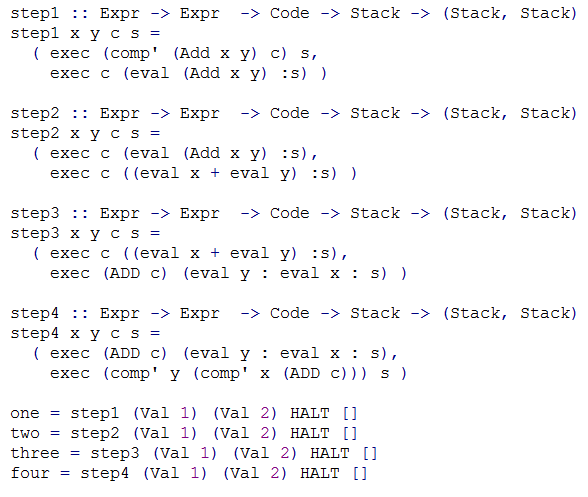
\includegraphics[scale=0.8]{Addsteps}
\caption{Steps from the calculation of \add}
\label{figadd}
\end{figure}

Compiling this in GHC passes, which means that
every one of those function is type correct and
therefore so are the steps of the \add\ calculation.

What's more is that we can invoke each of these steps
with an expression 
\( \Add (\Val 1)\ (\Val 2) \)
 and show that they still hold true
because they will all produce the same answer pair
\begin{eqnarray*}
\mathit{one} &\rightarrow& ([3], [3]) \\
\mathit{two} &\rightarrow& ([3], [3]) \\
\mathit{three} &\rightarrow& ([3], [3]) \\
\mathit{four} &\rightarrow& ([3], [3]) \\
\end{eqnarray*}

In later subsections
this array of arrows will be shortened to
\( \mathit{one,\ two,\ three,\ four } \rightarrow ([3], [3]) \)
to indicate that all invocations of steps before 
the arrow agree on the answer after the arrow.

\subsection{Conditionals, $L_c$}

Here are the step functions in Haskell which model the
steps of calculation in \S\ref{itecalc}
\begin{figure}[h] 
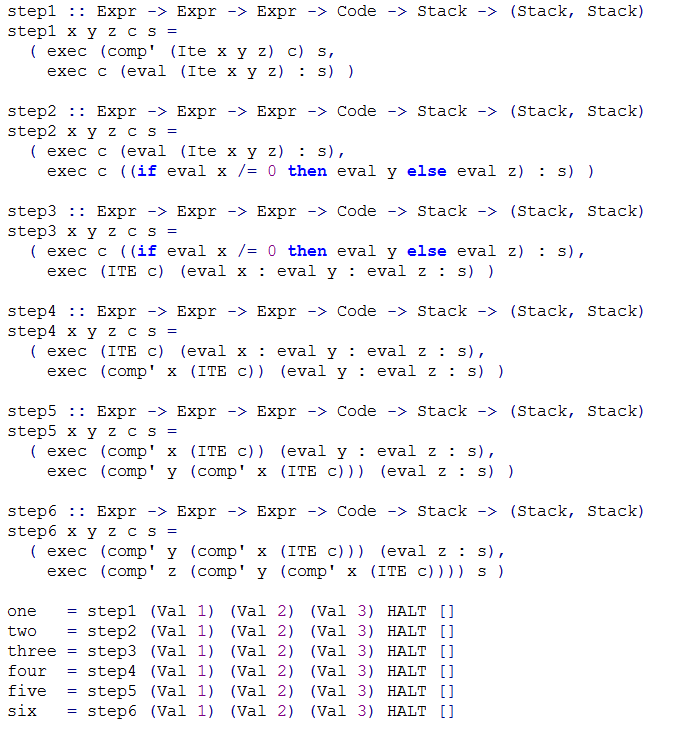
\includegraphics[scale=0.8]{Itesteps}
\caption{Steps from the calculation of \ite}
\label{figite}
\end{figure}

(See figure \ref{figite})
GHC shows that each step is type correct by 
successfully compiling the program, 
and
therefore so are the steps in the \ite\ calculation.

Invoking each of these steps
with an example 
\( \Ite (\Val 1)\ (\Val 2)\ (\Val 3) \)
shows that they still hold true
because they all produce the same answer pair
\begin{equation*}
\mathit{one,\ two,\ three,\ four,\ five,\ six } 
		\rightarrow ([2], [2]) \\
\end{equation*}

\subsection{Lazy conditionals, $L_c$}

Step functions in Haskell modelling the
steps of calculation in \S\ref{lazycon}:
\begin{figure}[h]
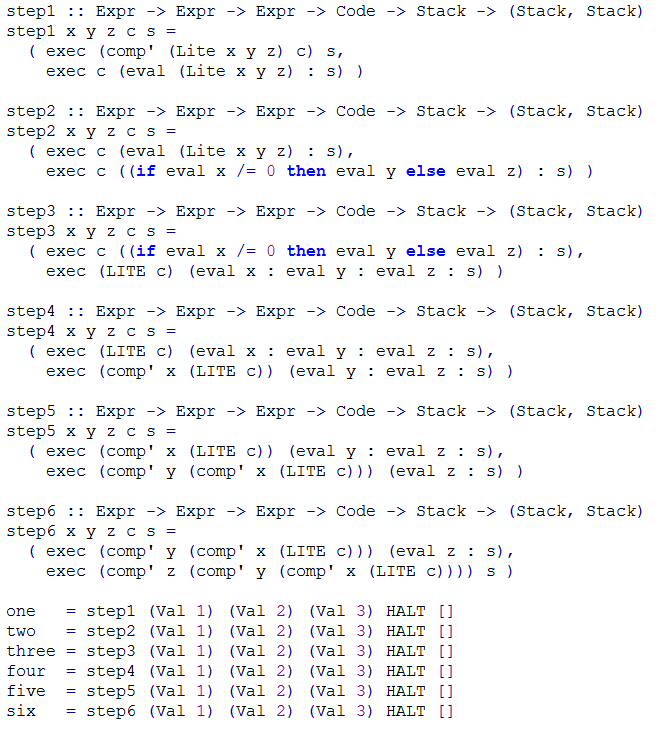
\includegraphics[scale=0.8]{Litesteps}
\caption{Steps from the calculation of \lite}
\label{figlite}
\end{figure}

(See figure \ref{figlite})
GHC shows that each step function 
and therefore the 
steps in the \lite\ calculation is type correct
by successfully compiling the program.

Invoking each of these steps
with an example 
\( \Lite (\Val 1)\ (\Val 2)\ (\Val 3) \)
shows that they still hold true
because they all produce the same answer pair
\begin{equation*}
\mathit{one,\ two,\ three,\ four,\ five,\ six } 
		\rightarrow ([2], [2]) \\
\end{equation*}

\subsection{Variable bindings, $L_b$}

In this series of tests the code is a bit more
complicated because of the new data structures:
\Cxtt\ and \textit{Memory}, but the over all
idea and purpose remains the same. More importantly
and less noticeably, we need to use the identity
of \zip\ (\ref{zcxtvs}), to keep the code within
width of the page sometimes $bs$ substituted
$(\Zip \Cxt \mathit{vs})$ but they are exactly the same.

Step functions in Haskell modelling the
steps of calculation in \S\ref{bindcal}:
\begin{figure}[h]
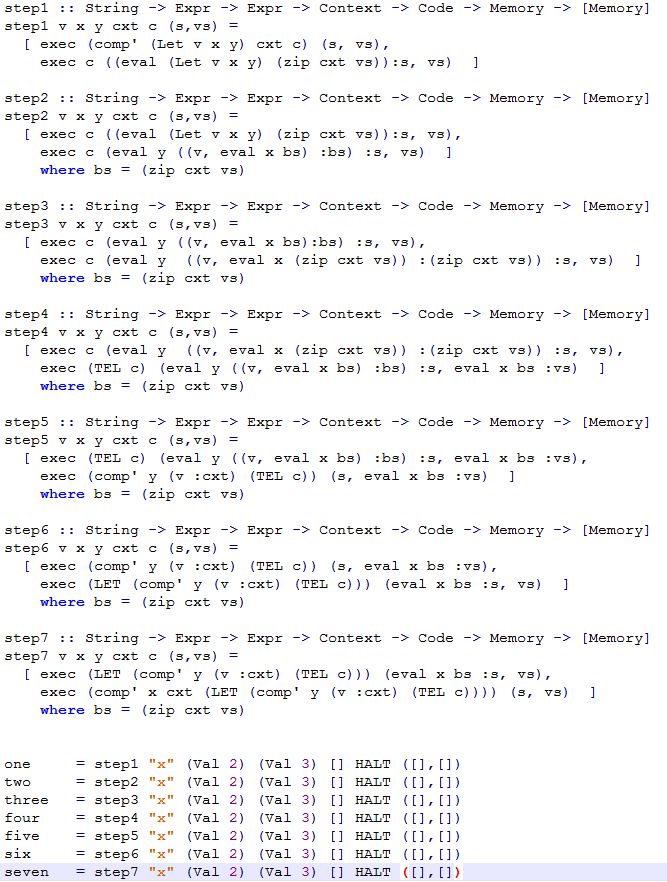
\includegraphics[scale=0.8]{Letsteps}
\caption{Steps from the calculation of \leet}
\label{figlet}
\end{figure}

(see figure \ref{figlet})
Compiling the program successfully, yet again,
GHC has shown that the step functions
and therefore the 
steps in the \leet\ calculation is type correct

Invoking each of these steps
with an example 
\( \Lite (\Val 1)\ (\Val 2)\ (\Val 3) \)
shows that they still hold true
because they all produce the same answer pair
\begin{equation*}
\mathit{one,\ two,\ three,\ four,\ five,\ six,\ seven } 
		\rightarrow [([3], []),([3], [])] \\
\end{equation*}

\subsection{Lazysmallcheck}

This subsection will conclude our automated testing
with the application of the Haskell library
``Lazysmallcheck''.

This library generates and tests multitudes of source 
code of varying lengths and increasing depths
against a certain property, should any source 
code not satisfy the property then the whole test fails.
The property in our case is that 
every expression should be well scoped,
and if it is well scoped then
it should satisfy the compiler correctness equation.
The test has been limited to choosing only values
1 and 2, and variables ``x'' and ``y'',
this is so the growth rate of possible source code
doesn't explode as immediately.

The results of Running this test in the library
produces the results:
(see figure \ref{lsch})
\begin{figure}[h]
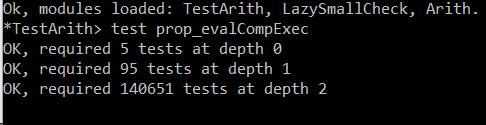
\includegraphics[scale=0.8]{ghctest}
\caption{Lazysmallcheck test results}
\label{lsch}
\end{figure}


Our tests could only reach a depth of 2 because
the growth rate of all possible source code
is still massive even with the limitations,
as you can see from the fact that there is a
jump in 14,0556 tests between depths 1 and 2.

But we can conclude from this that our 
compiler and \vm\ have produced a language
that can at least hold up to depths of two.
With more limitations on the testing we
could get to deeper depths, however
we would need to consider the trade off
in that the 
limitations might prevent us from finding 
a failure case, and thus let a bug fly by.

\pagebreak
\section{Conclusion} \label{conclusion}

In conclusion these \BH\ method has proved itself both
relatively straightforward to use and flexible.
We managed to stay true to the method throughout 
our calculations and in doing so found ourselves often in familiar
situations, most notably from how the calculations would
stop at the same point. Getting into these familiar spots
was helpful because they meant that 
previous experience could be used and built upon which made
it easier to progress, this was apparent in \S\ref{lazycon}
when we wanted to invent a definition for \exec\ for \lite\.
Even in the thick and complicated calculation of \let\ we 
did not need to deviate from the method.

Difficulty comes when the semantics of the source
expression demand for additional data structures,
as we saw in \S\ref{langbind}, the real challenge 
arises from connecting these data structures
from compiler to the semantics via the \vm,
however it has been found that the struggle is very much
worthwhile because the definitions that fall out of the
process are robust and hold up to testing.

Further work can certainly explore calculations
into function declaration, 
from what has been seen in this paper,
it is not hard to imagine that the calculation would 
put the \BH\ method under stress, but 
(it is hypothesised that) there would be
numerous learning outcomes in better understanding of 
using induction hypotheses.
Furthermore we touched upon optimisation in
\S\ref{lazycon} as issue. Perhaps study into
this area might reveal more ways to improve the 
\BH\ method on top of the refinements they made
throughout their paper\cite{bandh}.



\bibliographystyle{IEEEtran}
\bibliography{Finalproject}
\end{document}